\documentclass[14pt, a4paper]{article}
\usepackage{minitoc}
\usepackage[left=3.00cm, right=2.5cm, top=2.00cm, bottom=2.00cm]{geometry}
\usepackage{amsmath}
\usepackage{amssymb}
\usepackage{amsthm}
\usepackage{mathtools}
\usepackage{graphicx}
\usepackage{algpseudocode}
\usepackage{algorithm}
\usepackage{blindtext}
\usepackage{setspace}
\usepackage[utf8]{inputenc}
\usepackage[utf8]{vietnam}
\usepackage[center]{caption}
\usepackage[shortlabels]{enumitem}
\usepackage{fancyhdr} % header, footer
\usepackage{hyperref} % loại bỏ border với mục lục và công thức
\usepackage[nonumberlist, nopostdot, nogroupskip]{glossaries}
\usepackage{glossary-superragged}
\setglossarystyle{superraggedheaderborder}
\pagestyle{fancy}
%\usepackage[style=numeric,sortcites]{biblatex}
%\addbibresource{ref.bib}
%\usepackage[numbers]{natbib}
\usepackage{indentfirst}
\usepackage[natbib,backend=biber,style=ieee, sorting=ynt]{biblatex}
\bibliography{ref.bib}

\graphicspath{{./figures/}}

\makenoidxglossaries

% Danh mục thuật ngữ

\newglossaryentry{RNN}
{
	name={RNN},
	description={Recurrent Neural Network}
}

\newglossaryentry{LSTM}
{
	name={LSTM},
	description={Long Short Term Memory}
}

\newglossaryentry{GRU}
{
	name={GRU},
	description={Gated Recurrent Unit}
}

\newglossaryentry{BERT}
{
	name={BERT},
	description={Bidirectional Encoder Representations from Transformer}
}

\newglossaryentry{BLEU}
{
	name={BLEU},
	description={Bilingual Language Evaluation Understudy}
}

\newglossaryentry{CNN}
{
	name={CNN},
	description={Convolutional Neural Networks}
}

\newglossaryentry{MLP}
{
	name={MLP},
	description={Multilayer Perceptron}
}

\newglossaryentry{NWGM}
{
	name={NWGM},
	description={Normalized Weighted Geometric Mean}
}

\newglossaryentry{GAP}
{
	name={GAP},
	description={Geometric Average Precision}
}

\newglossaryentry{GUI}
{
	name={GUI},
	description={Graphical User Interface}
}

\hypersetup{
    colorlinks=false,
    pdfborder={0 0 0},
}

\title{Báo cáo bài tập lớn môn học}

\author{Nguyễn Chí Thanh}


\fancyhf{}
\rhead{\textbf{Phát triển phần mềm nâng cao cho tính toán khoa học}}
\lhead{\textbf{GVHD: TS. Vũ Tiến Dũng}}
\rfoot{\thepage}
\lfoot{\textbf{Ứng dụng Deep Learning cho tự động sinh mô tả ảnh}}
\renewcommand{\headrulewidth}{0.4pt}
\renewcommand{\footrulewidth}{0.4pt}

\numberwithin{equation}{section}
\numberwithin{algorithm}{section}
\numberwithin{figure}{section}
\numberwithin{table}{section}

\setlength{\parindent}{0.5cm}

\setcounter{secnumdepth}{3} % Cho phép subsubsection trong report
\setcounter{tocdepth}{3} % Chèn subsubsection vào bảng mục lục

\newtheorem{dl}{Định lý}
\newtheorem{md}{Mệnh đề}
\newtheorem{bd}{Bổ đề}
\newtheorem{dn}{Định nghĩa}
\newtheorem{hq}{Hệ quả}

\numberwithin{dl}{section}
\numberwithin{md}{section}
\numberwithin{bd}{section}
\numberwithin{dn}{section}
\numberwithin{hq}{section}

\doublespacing

\begin{document}
    \cleardoublepage
    \pagenumbering{gobble}
    \tableofcontents
    \newpage
    \listoffigures
    \newpage
    \listoftables
    \newpage
    \glsaddall 
    \renewcommand*{\glossaryname}{Danh mục từ viết tắt}
    %\renewcommand*{\glossaryname}{Danh mục thuật ngữ}
    %\renewcommand*{\acronymname}{Danh sách từ viết tắt}
    %\renewcommand*{\entryname}{Viết tắt}
    %\renewcommand*{\descriptionname}{Viết đầy đủ}
    \printnoidxglossary
    \cleardoublepage
    \pagenumbering{arabic}

    %\maketitle

    \newpage

    \nocite{*}

    \begin{center}
    \section*{LỜI MỞ ĐẦU}
    \end{center}
    \addcontentsline{toc}{section}{{\bf LỜI MỞ ĐẦU}\rm}

    Hiện nay với sự phát triển của các mạng xã hội, lượng ảnh và thông tin được tải lên với số lượng ngày một nhiều, điều này tạo ra một thách thức trong việc hiểu cũng như kiểm duyệt nội dung các ảnh mà người dùng tải lên.
    Để thực hiện được các công việc này cần phải có những công cụ tự động có tốc độ và hiệu quả cao. Cũng vì vậy mà các phương pháp về trí tuệ nhân tạo nói chung và học máy (\textit{Machine Learning}) nói chung đã phát triển rất mạnh mẽ và có nhiều bước đột phá.

    Một trong số đó có thể kể đến các mô hình Vision-Language là các mô hình có sự kết hợp giữa các thể thức ảnh và ngôn ngữ tự nhiên. Một mô hình tiêu biểu trong số các mô hình Vision-Language không thể không nhắc đến mô hình sinh mô tả ảnh.
    Mô hình sinh mô tả ảnh có rất nhiều ứng dụng như: Gán nhãn tự động cho ảnh, Hỗ trợ người thị lực kém hoặc người khiếm thị xác định cảnh vật xung quanh hoặc hỗ trợ di chuyển hoặc tìm kiếm ảnh dựa trên mô tả.

    Ngoài mô hình sinh mô tả ảnh còn có một số các mô hình phổ biến khác trong nhóm các mô hình Vision-Language như: Visual Grounding, Scene Graph Generation, Visual Question Answering, Text to Image Retrieval, ...
    Nhưng các mô hình trên không nằm trong phạm vi của đề tài.

    Kếu cấu của đề tài gồm 5 phần:

    \begin{itemize}
        \item Tổng quan về bài toán sinh mô tả ảnh
        \item Chi tiết mô hình
        \item Phương pháp đánh giá
        \item Thực nghiệm và kết quả
        \item Demo giao diện
        \item Kết luận và hướng phát triển đề tài
    \end{itemize}

    \newpage

    \section{Tổng quan về bài toán sinh mô tả ảnh}

    \subsection{Bài toán dịch máy (\textit{Machine Translation})} \label{Machine-Translation}
    Bài toán sinh mô tả ảnh là một bài toán rất thường gặp trong các ứng dụng của Deep Learning.
    Do đầu ra của bài toán sinh mô tả ảnh là ngôn ngữ, nên có thể xem mô hình sinh mô tả ảnh thuộc lớp mô hình xử lý ngôn ngữ tự nhiên.
    Vì vậy, kiến trúc của mô hình sinh mô tả ảnh kế thừa chủ yếu từ bài toán dịch máy (\textit{Machine Translation}).
    
    Bài toán dịch máy là việc dịch tự động một đoạn văn bản từ ngôn ngữ này sang ngôn ngữ khác.
    Giải quyết bài toán với các mạng neuron được gọi là dịch máy neuron (\textit{Neural Machine Translation}).
    Dịch máy có ứng dụng rất lớn trong đời sống xã hội cũng như phục vụ công tác nghiên cứu khoa học. 
    Một phần mềm nổi bật nhất về bài toán dịch máy rất phổ biến hiện nay là Google dịch (\textit{Google Translate}).
    
    Dịch máy là một bài toán rất được quan tâm bởi cộng đồng xử lý ngôn ngữ tự nhiên (\textit{Natural Language Processing}) đặc biệt là dịch máy neuron đã đạt được rất nhiều bước tiến trong những năm vừa qua.
    Cấu trúc của một mô hình dịch máy neuron điển hình gồm hai thành phần chính:

    \begin{itemize}
        \item Thành phần mã hóa (\textit{Encoder}): Thành phần này có nhiệm vụ mã hóa câu đầu vào thuộc ngôn ngữ nguồn thành một vector. Vector này trở thành đầu vào hoặc được biến đổi trở thành trạng thái đầu của thành phần tiếp theo.
        \item Thành phần giải mã (\textit{Decoder}): Thành phần này nhận vector đầu ra từ thành phần encoder, biến đổi vector này thành đầu vào hoặc trạng thái đầu của thành phần này. Đầu ra của thành phần này là các từ trong ngôn ngữ đích. Quá trình đưa ra từng từ trong ngôn ngữ đích được gọi là quá trình dịch.
    \end{itemize}

    \begin{figure}[h!] \centering

        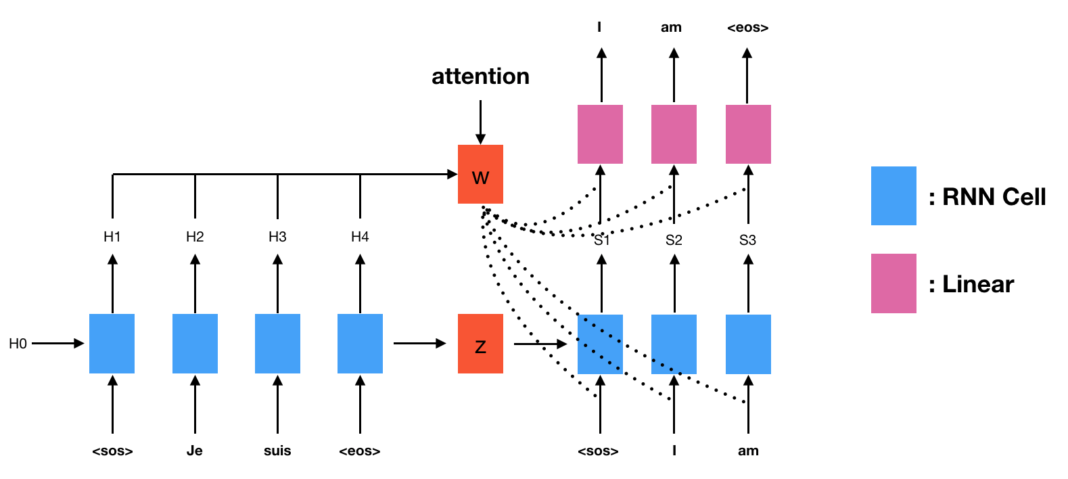
\includegraphics[scale=0.35]{Neural_Machine_Translation_Architecture.png}
        \caption{Cấu trúc chung của một mô hình dịch máy neuron.}
    
        \label{fig:Neural_Machine_Translation_Architecture}
    \end{figure}

    Một cấu trúc điển hình của một mô hình dịch máy neuron được minh họa ở hình \ref{fig:Neural_Machine_Translation_Architecture}.
    Ngoài hai thành phần quan trọng kể trên, còn có một thành phần quan trọng khác không bắt buộc nhưng rất hay xuất hiện ở trong các mô hình dịch máy là thành phần sử dụng cơ chế tập trung (\textit{Attention}).
    Một số công trình mà mô hình đóng một vai trò quan trọng: \cite{bahdanau2014neural}, \cite{luong2014addressing}, \cite{jean2014using}, \cite{luong2015effective}, \cite{tang2016neural}, \cite{wang2016memory}, \cite{li2016towards}, \cite{tu2016modeling}, \cite{shen2015minimum}, \cite{zhou2016deep}.

    Cơ chế Attention bản chất chính là sự chú ý. Trong quá trình dịch, mô hình sẽ cần tập trung vào từ nào ở trong câu đầu vào để đưa ra lựa chọn từ nào ở trong ngôn ngữ đích.
    Lý do cơ chế Attention ra đời là vì mô hình chỉ có hai thành phần encoder và decoder có một hạn chế rất lớn. Encoder sẽ phải nén toàn bộ thông tin của câu đầu vào thành một vector, rõ ràng đây không phải là điều hợp lý.
    Đặc biệt khi câu đầu vào dài thì enocder phải đưa toàn bộ các thông tin vào một vector thì nó sẽ phải làm mất hoặc quên một thông tin nào đó.
    Mặt khác, thành phần decoder chỉ thấy một vector biểu diễn đầu vào duy nhất, dù mỗi bước thời gian (\textit{timestep}) khác nhau thì các thành phần khác nhau của câu đầu vào có ích hơn phần khác.
    Nhưng nếu chỉ có một vector duy nhất, việc để chọn ra thông tin hợp lý tại mỗi timestep gần như không khả thi.

    Hai cơ chế Attention hay được sử dụng phổ biến nhất là Bahdanau Attention \cite{bahdanau2014neural} và Luong Attention \cite{luong2014addressing}. Trong bài tập lớn, nhóm sẽ chỉ sử dụng và trình bày Bahdanau Attention.
    Ta giả sử có một câu đầu vào $\bold{X}$ với độ dài là $L$ từ, và một câu dịch tương ứng $\bold{Y}$ với độ dài $C$ từ:

    \begin{equation}
        \begin{aligned}
            \bold{X} = \lbrack \bold{x}_1, \bold{x}_2, \dots, \bold{x}_L \rbrack, \bold{x}_i \in \mathbb{R}^D \\
            \bold{Y} = \lbrack \bold{y}_1, \bold{y}_2, \dots, \bold{y}_C \rbrack, \bold{y}_t \in \mathbb{R}^K
        \end{aligned}
    \end{equation}

    Một từ trong một timestep $t$ của thành phần đầu ra của decoder phụ thuộc vào đầu ra timestep phía trước $\bold{y}_{t-1}$, trạng thái ẩn của decoder $\bold{h}_t$ và vector bối cảnh $\bold{z}_t$ được tính theo công thức tổng quát:

    \begin{equation}
        p(\bold{y}_t \vert \lbrace \bold{y}_1, \bold{y}_2, \dots, \bold{y}_{t-1} \rbrace, \bold{X}) = g(\bold{y}_{t-1}, \bold{h}_t, \bold{z}_t)
    \end{equation}

    Trạng thái ẩn $\bold{h}_t$ của decoder được tính một mạng RNN với thông tin từ trạng thái ẩn của timestep trước, đầu ra của bước trước và vector bối cảnh:
    
    \begin{equation}
        \bold{h}_t = f(\bold{y}_{t-1}, \lbrace \bold{c}_{t-1}, \bold{h}_{t-1} \rbrace, \bold{z}_t) \forall t=1,\dots,C
    \end{equation}

    Vector bối cảnh là vector được tính bằng tổng trọng số của đầu ra của encoder tại đầu thứ $i$, $\alpha_{ti}$ biểu thị trọng số mức độ chú ý với đầu ra $\bold{a}_i$ ở timestep thứ $t$:

    \begin{equation}
        \bold{z}_t = \sum_{i=1}^{L}\alpha_{ti}\bold{a}_i
    \end{equation}

    Với $\alpha_{ti}$ thực chất được tính từ hàm softmax là trọng số riêng được tính từ đầu ra thứ $i$ của encoder. Hàm softmax là một cách để chuẩn hóa các $\alpha_{ti}$ cho $\sum_{i=1}^{L}\alpha_{ti}=1$

    \begin{equation}
        \alpha_{ti} = \dfrac{e_{ti}}{\sum_{k=1}^{L} e_{tk}}
    \end{equation}

    $e_{ti}$ là tương quan giữa đầu ra $\bold{y}_t$ bước thứ $t$ và đầu vào $\bold{x}_i$ bước thứ $i$ thường được tính bằng một mạng neuron:

    \begin{equation}
        e_{ti} = f_{\text{att}}(\lbrace \bold{c}_{t-1}, \bold{h}_{t-1} \rbrace, \bold{a}_i)
    \end{equation}

    Trong \cite{bahdanau2014neural}, tác giả đề xuất một Attention model với công thức:

    \begin{equation}
        e_{ti} = f_{\text{att}}(\lbrace \bold{c}_{t-1}, \bold{h}_{t-1} \rbrace, \bold{a}_i) = \bold{v}_{\bold{a}}^T \tanh (\bold{W} \lbrace \bold{c}_{t-1}, \bold{h}_{t-1} \rbrace + \bold{U}\bold{a}_i)
    \end{equation}

    với $\bold{W} \in \mathbb{R}^{2D \times D}$ và $\bold{U}^{D \times D}$, $\bold{v}_{\bold{a}} \in \mathbb{R}^{D}$ là các ma trận trọng số được huấn luyên.

    Thực chất cơ chế Attention giúp cho mô hình tập trung vào các phần quan trọng của dữ liệu, bằng việc tạo một mạng neuron đơn giản tính các trọng số $\alpha_{ti}$ để đánh lại các trọng số của các đầu ra của encoder $\bold{a}_i$.
    Trong mô hình dịch máy neuron, việc này giúp mô hình tập trung hơn vào những từ quan trọng trong câu đầu vào $\bold{X}$, từ đó dự đoán ra từ $\bold{y}_t$ tiếp theo tại decoder, được biểu diễn bằng các ô sáng màu trong Attention map ở hình \ref{fig:Attention_Map}

    \begin{figure}[h!] \centering

        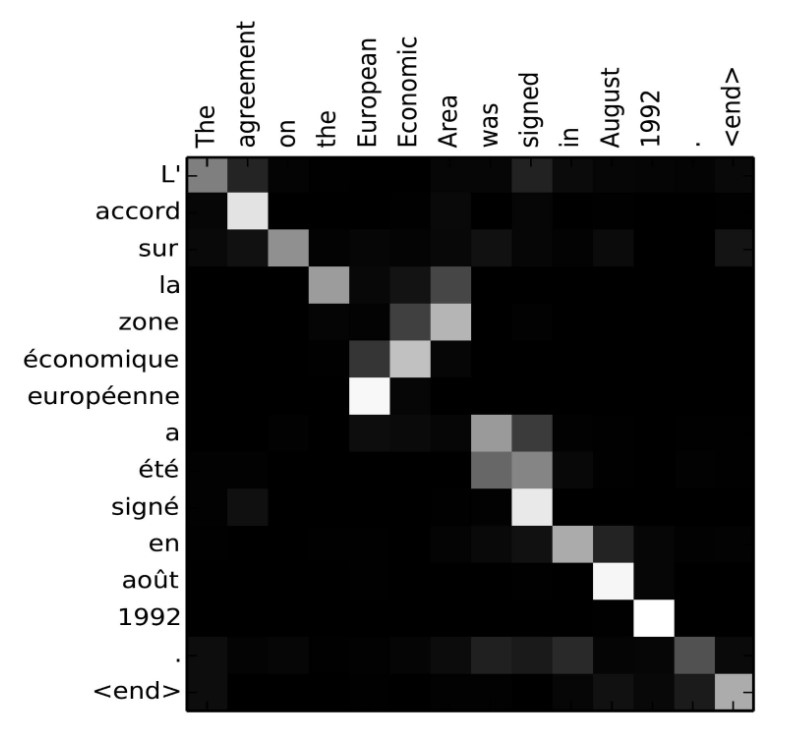
\includegraphics[scale=0.5]{Attention_Map.jpg}
        \caption{Ma trận biểu diễn mức độ tương quan giữa từng từ ở câu đầu vào (tiếng Pháp) và câu được dịch đầu ra (tiếng Anh).}
    
        \label{fig:Attention_Map}
    \end{figure}

    Một số cơ chế tính Attention khác:

    \begin{itemize}
        \item Content-base Attention: $e_{ti}=\cos(\lbrace \bold{c}_{t-1}, \bold{h}_{t-1} \rbrace, \bold{a}_i)$ được đề xuất trong \cite{graves2014neural}
        \item Additive Attention chính là cơ chế Attention được trình bày ở trên \cite{bahdanau2014neural}
        \item Dot-Product Attention được đề xuất trong \cite{luong2015effective}
        \item General Attention được đề xuất trong \cite{luong2015effective}
    \end{itemize}

    Ngoài ra còn một số các loại cơ chế Attention khác:

    \begin{itemize}
        \item Self-Attention.
        \item Soft/Hard Attention.
        \item Global/Local Attention.
    \end{itemize}

    \textbf{Self-Attention:} là một cơ chế Attention chỉ dùng cho một câu. 
    Ta sẽ tự tạo một ma trận tương quan giữa từng từ trong câu để hiểu những phần nào của câu sẽ liên quan đến nhau.
    Cơ chế này đã chứng minh được sự hiệu quả trong các bài toán xử lý ngôn ngữ tự nhiên như tóm tắt văn bản, dịch máy,... 
    Cùng với self-attention là sự ra đời của cấu trúc Transformer \cite{vaswani2017attention} cho phép thay thế hoàn toàn kiến trúc mạng neuron RNN bằng các mô hình kết nối đầy đủ (\textit{fully connected}) mà vẫn cho kết quả tốt.


    \textbf{Soft/Hard Attention:} Hai cơ chế này được áp dụng cho bài toán sinh mô tả ảnh.
    Ảnh đầu tiên sẽ được trích xuất đặc trưng qua mạng neuron tích chập CNN (\textit{Convolutional Neural Networks}) sau đó mạng LSTM kết hợp với cơ chế Attention sẽ thực hiện nhiệm vụ giải mã (\textit{decoding}) các đặc trưng để tạo ra mô tả cho ảnh.
    Hai cơ chế Soft Attention và Hard Attention được phân biệt như sau:

    \begin{itemize}
        \item \textbf{Soft Attention:} sử dụng các trọng số $\alpha_{ti}$ để tính ra vector bối cảnh và nó là hàm khả vi nên có thể sử dụng giảm theo gradient (\textit{Gradient Descent}) và lan truyền ngược (\textit{Back Propagation}) để huấn luyện. 
        Tuy nhiên do tính trên toàn bộ đầu vào thì đối với các bài toán liên quan đến ảnh thì chi phí tính toán sẽ rất cao khi kích thước ảnh lớn.
        \item \textbf{Hard Attention:} thay vì tính trung bình có trọng số của tất cả các vector đầu ra của encoder thì sử dụng điểm Attention để lựa chọn vị trí của vector thích hợp nhất.
        Hard Attention thường được huấn luyện bằng các phương pháp học tăng cường (\textit{Reinforcement Learning}). Ưu điểm của cơ chế này là chi phí tính toán thấp hơn, nhưng yêu cầu kỹ thuật phức tạp để huấn luyện.
    \end{itemize}

    \textbf{Global/Local Attention:} Các mô hình mặc định hay dùng cơ chế Global Attention là cơ chế Attention sẽ tính toán dựa trên toàn bộ đầu vào.
    Nhưng các bài toán đôi khi có thể có chi phí tính toán tốn kém hoặc không cần thiết. Do vậy một số mô hình đưa ra cơ chế Local Attention, chỉ quan tâm đến một phần của đầu vào.
    Local Attention có thể coi giống như Hard Attention. Ngoài ra có thể so sánh Global Attention như một mạng fully connected, còn Local Attention thì giống như mạng neuron tích chập CNN.
    Hình \ref{fig:Local_Global_Attention} so sánh sự khác biệt giữa hai cơ chế Attention.

    \begin{figure}[h!] \centering

        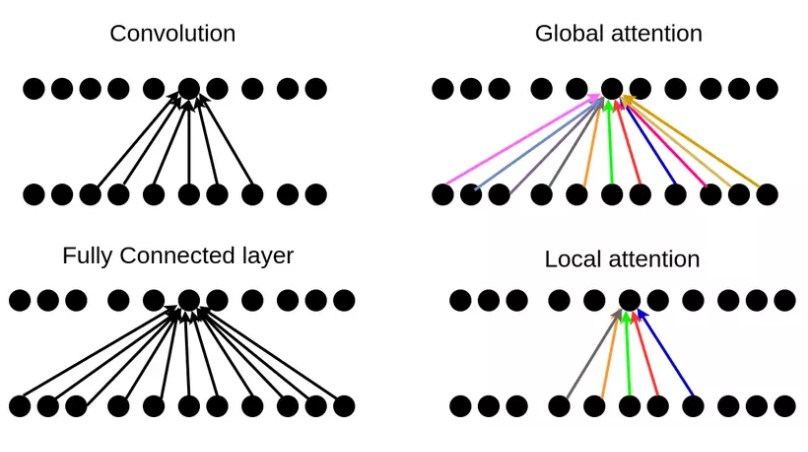
\includegraphics[scale=0.4]{Local_Global_Attention.jpg}
        \caption{So sánh hai cơ chế Global Attention và Local Attention}
    
        \label{fig:Local_Global_Attention}
    \end{figure}

    \subsection{Bài toán sinh mô tả ảnh}

    Ở mục \ref{Machine-Translation} ta đã giới thiệu tổng quan về cấu trúc của một mô hình dịch máy và cơ chế Attention. 
    Ở mục này ta sẽ giới thiệu cấu trúc của một mô hình sinh mô tả ảnh. 
    Cấu trúc của một mô hình sinh mô tả ảnh được minh họa trong hình \ref{fig:Image_Captioning_Architecture}

    \begin{figure}[h!] \centering

        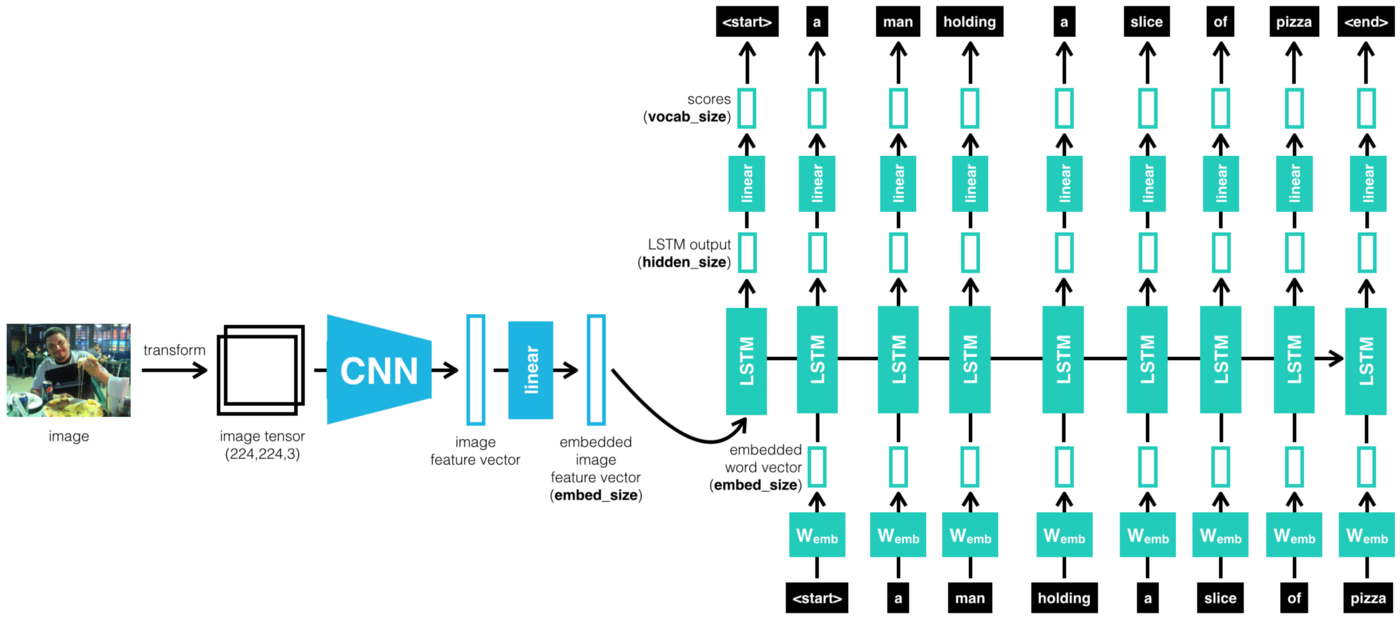
\includegraphics[scale=0.25]{Image_Captioning_Architecture.png}
        \caption{Cấu trúc của một mô hình sinh mô tả ảnh}
    
        \label{fig:Image_Captioning_Architecture}
    \end{figure}

    Do cũng giống như một bài toán dịch máy, mô hình sinh mô tả ảnh cũng giống như mô hình dịch máy gồm hai thành phần chính là Encoder và Decoder.
    Nhưng khác ở chỗ, vì đầu vào của mô hình sinh mô tả ảnh là ảnh nên cấu trúc của Encoder của mô hình mô tả ảnh sẽ khác so với Encoder của mô hình dịch máy.
    Encoder trong mô hình sinh mô tả ảnh thường là một CNN hoặc một mô hình Deep Learning xử lý ảnh (ví dụ: Vision Transformer \cite{dosovitskiy2020image}).
    Còn lại cấu trúc của Decoder của mô hình sinh mô tả ảnh giống như Decoder của mô hình dịch máy.

    Ban đầu một ảnh được đưa vào Encoder, đầu ra sẽ tạo ra một vector hoặc một tập các vector (như ở bài toán dịch máy).
    Các vector này sẽ trở thành đầu vào của Decoder phục vụ cho quá trình dịch.
    Mô hình sinh mô tả ảnh cũng rất hay sử dụng cơ chế Attention. 
    Vì khi thực hiện quá trình dịch để tạo ra mô tả ảnh, tại mỗi timestep, mô hình cần tập trung đến khu vực nào của ảnh để chọn ra một từ phù hợp.

    Mô hình CNN hay được sử dụng là một Pretrained Model đã được huấn luyện trên tập dữ liệu ImageNet. 
    Đây là kỹ thuật Transfer Learning rất hay được sử dụng trong các bài toán thị giác máy tính (\textit{Computer Vision}), được dùng để tận dụng một mô hình được huấn luyện trên tập dữ liệu này cho một tập dữ liệu khác.
    Các mô hình CNN áp dụng cho các mô hình sinh mô tả ảnh được không được huấn luyện hoặc được huấn luyện một vài lớp neuron cuối.

    \section{Chi tiết mô hình}

    \subsection{Encoder}

    Mô hình nhận vào là một ảnh và tạo ra mô tả ảnh $\bold{y}$ được biểu diễn dưới dạng $K$ từ:

    \begin{equation}
        \bold{y} = \lbrace \bold{y}_1, \dots, \bold{y}_C \rbrace, \bold{y}_i \in \mathbb{R}^K
    \end{equation}

    với $K$ là số từ trong từ điển và $C$ là độ dài của câu mô tả ảnh.
    
    Encoder là một mô hình CNN tạo ra một tập các vector đặc trưng được gọi là các \textit{vector gán nhãn}.
    Encoder trích xuất ra $L$ vector gán nhãn ứng với mỗi ảnh, mỗi vector gán nhãn có số chiều là $D$.
    Mỗi vector gán nhãn tương ứng với một vùng hình ô vuông ở trong ảnh.

    \begin{equation}
        \bold{a}=\lbrace \bold{a}_1, \dots, \bold{a}_L \rbrace, \bold{a}_i \in \mathbb{R}^D
    \end{equation}

    Để thu được các vector gán nhãn tương ứng với các vùng của ảnh, mô hình lấy vector từ lớp tích chập (\textit{convolutional layer}) thay vì lấy vector từ lớp fully connected.
    Điều này cho phép Decoder lựa chọn tập trung vào một vùng nhất định bằng cách lựa chọn một tập con của các vector gán nhãn.

    \subsection{Decoder}

    Decoder sử dụng LSTM \cite{hochreiter1997long} tạo ra câu mô tả ảnh theo từng từ theo từng timestep dựa trên vector bối cảnh $\bold{z}_t$, trạng thái ẩn của bước trước $\bold{h}_{t-1}$ và từ được sinh ra ở bước trước $\bold{y}_{t-1}$.

    \subsubsection{Kiến trúc LSTM}

    Kiến trúc LSTM được ra đời để khắc phục những nhược điểm của kiến trúc RNN truyền thống.
    Một nhược điểm lớn nhất của RNN là hiện tượng Gradient bị triệt tiêu (\textit{vanishing gradient}) hoặc Gradient bị bùng nổ (\textit{exploding gradient}).
    Do trong quá trình huấn luyện RNN, các trọng số của RNN được học bằng cách tính đạo hàm riêng phải thông qua chuỗi thời gian, nếu mỗi đạo hàm riêng theo từng timestep nhỏ hơn 1, sau nhiều bước tích của nhiều số nhỏ hơn 1 trở thành 1 số rất nhỏ.
    Như vậy, các từ ở xa không còn tác dụng với từ hiện tại nữa, làm cho RNN không thể học jđược các phụ thuộc xa.


    \begin{figure}[h!] \centering

        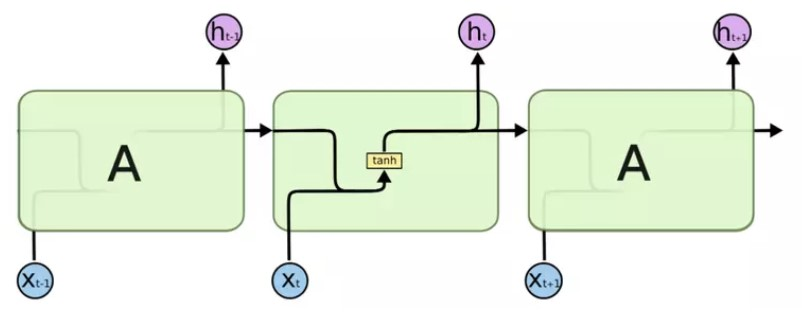
\includegraphics[scale=0.9]{RNN_Sequence.jpg}
        \caption{Kiến trúc RNN}
    
        \label{fig:RNN_Sequence}
    \end{figure}

    \begin{figure}[h!] \centering

        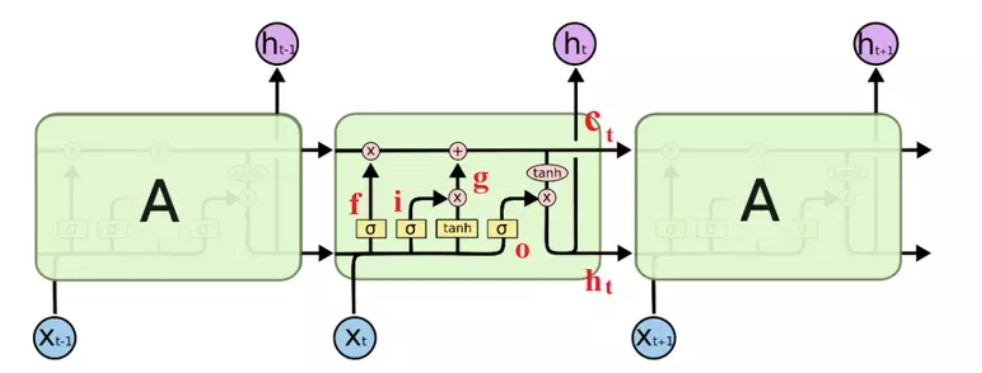
\includegraphics[scale=0.8]{LSTM_Sequence.jpg}
        \caption{Kiến trúc LSTM}
    
        \label{fig:LSTM_Sequence}
    \end{figure}

    Sự so sánh kiến trúc RNN và kiến trúc LSTM được minh họa ở hình \ref{fig:RNN_Sequence} và \ref{fig:LSTM_Sequence}.
    Về cơ bản ý tưởng không khác nhau là mấy.

    Công thức tính trạng thái ẩn của RNN là:

    \begin{equation}
        \bold{h}_t = \tanh \Bigg( W_{\mathrm{RNN}} \begin{bmatrix} \bold{h}_{t-1} \\ \bold{x}_t \end{bmatrix} \Bigg)
    \end{equation}

    Và công thức cho LSTM:

    \begin{equation}
        \begin{cases}
            \begin{bmatrix}
                \bold{i}_t \\
                \bold{f}_t \\
                \bold{o}_t \\
                \bold{g}_t
            \end{bmatrix}=\begin{bmatrix}
                \sigma \\
                \sigma \\
                \sigma \\
                \mathrm{tanh}
            \end{bmatrix}W_{\mathrm{LSTM}}\begin{bmatrix}
                \bold{h}_{t-1} \\
                \bold{x}_t
            \end{bmatrix} \\
            \bold{c}_t = \bold{f}_t \odot\bold{c}_{t-1} + \bold{i}_t \odot \bold{g}_t \\
            \bold{h}_t = \bold{o}_t \odot \mathrm{tanh}(\bold{c}_t)
        \end{cases}
    \end{equation}

    Đầu tiên, ta có $\bold{i}_t, \bold{f}_t, \bold{g}_t$ có công thức gần giống hệt nhau và chỉ khác mỗi ma trận tham số. 
    Chính ma trận này sẽ quyết định chức năng khác nhau của từng cổng.
    $\sigma$ là ký hiệu của hàm sigmoid.

    \begin{itemize}
        \item Cổng vào (\textit{Input gate}) $\bold{i}_t$: Cổng vào giúp quyết định bao nhiêu lượng thông tin đầu vào sẽ ảnh hưởng đến trạng thái mới. 
        Quyết định bằng cách  thông qua đặc điểm của hàm sigmoid (đầu ra nằm trong khoảng $\lbrack 0, 1\rbrack$), như vậy khi một vector thông tin đi qua đây, nếu nhân với 0, vector sẽ bị triệt tiêu hoàn toàn. Nếu nhân với 1, hầu hết thông tin sẽ được giữ lại.
        \item Cổng quên (\textit{Forget gate}) $\bold{g}_t$: Cổng quyết định sẽ bỏ đi bao nhiêu lượng thông tin đến từ trạng thái trước đó.
        \item Cổng ra (\textit{Output gate}) $\bold{o}_t$: Cổng điều chỉnh lượng thông tin có thể ra ngoài và lượng thông tin truyền tới trạng thái tiếp theo.
        \item Cổng $\bold{g}_t$ thực chất là một cổng trạng thái ẩn được tính dựa trên đầu vào hiện tại $\bold{x}_t$ và trạng thái trước $\bold{h}_{t-1}$.
        Cách tính giống hệt như cổng vào, nhưng sử dụng hàm kích hoạt là $\tanh$ thay vì sử dụng sigmoid, kết hợp với cổng vào để cập nhật trạng thái mới.
        \item $\bold{c}_t$ là bộ nhớ trong của LSTM, ta có thể thấy $\bold{c}_t$ là tổng hợp của bộ nhớ trước $\bold{c}_{t-1}$ đã được lọc qua cổng quên và trạng thái ẩn $\bold{g}_t$ đã được lọc qua cổng vào $\bold{i}_t$.
        Trạng thái này sẽ mang thông tin nào quan trọng truyền đi xa và được sử dụng khi cần.
        \item Sau đó trạng thái bộ nhớ $\bold{c}_t$ sẽ được đưa qua hàm kích hoạt $\tanh$ kết hợp với cổng ra $\bold{o}_t$ để thu được trạng thái mới $\bold{h}_t$.
    \end{itemize}

    Mô hình trong phương pháp sử dụng kiến trúc LSTM nhưng đầu vào $\bold{x}_t$ là kết hợp của từ được dịch ở bước trước $\bold{Ey}_{t-1}$ và vector bối cảnh $\hat{\bold{z}}_t$ với $\bold{E} \in \mathbb{R}^{m \times K}$ là một ma trận embedding từ của từ điển.
    $m$ và $n$ lần lượt là kích thước embedding và số chiều của trạng thái của LSTM:

    \begin{equation}
        \begin{cases}
            \begin{bmatrix}
                \bold{i}_t \\
                \bold{f}_t \\
                \bold{o}_t \\
                \bold{g}_t
            \end{bmatrix}=\begin{bmatrix}
                \sigma \\
                \sigma \\
                \sigma \\
                \mathrm{tanh}
            \end{bmatrix}T_{D+m+n,n}\begin{bmatrix}
                \bold{h}_{t-1} \\
                \bold{Ey}_{t-1} \\
                \hat{\bold{z}}_t
            \end{bmatrix} \\
            \bold{c}_t = \bold{f}_t \odot\bold{c}_{t-1} + \bold{i}_t \odot \bold{g}_t \\
            \bold{h}_t = \bold{o}_t \odot \mathrm{tanh}(\bold{c}_t)
        \end{cases}
    \end{equation}

    \subsubsection{Mô hình Attention}

    Ta sẽ thiết kế một cơ chế Attention $\phi$ để tính $\hat{\bold{z}}_t$ từ các vector gán nhãn $\bold{a}_i, i=1, \dots, L$ tương ứng với các đặc trưng được trích xuất với các phần khác nhau của ảnh đầu vào.
    Cho từng vị trí $i$, cơ chế Attention sẽ tạo ra một trọng số dương $\alpha_i$ biểu đạt xác suất mà vị trí thứ $i$ là vị trí được chú ý để tạo ra từ tiếp theo hoặc là trọng số tương đối của vị trí thứ $i$ để hợp nhất các vector $\bold{a}_i$ lại với nhau.
    Trọng số $\alpha_i$ của từng vector gán nhãn $\bold{a}_i$ được tính dựa vào một mô hình Attention $f_{\mathrm{att}}$ chỉ đơn giản là một mạng MLP (\textit{Multilayer Perceptron}) dựa vào trạng thái của bước trước $\bold{h}_{t-1}$.
    Một phiên bản phổ biến của Attention đã được đề xuất trong \cite{bahdanau2014neural}. Một điều cần chú ý là các trạng thái ẩn biến đổi theo từng bước, đầu ra của mô hình Attention nghĩa là mô hình sẽ tập trung vào đâu để tạo ra từ mới dựa vào những từ đã được tạo ra từ các bước trước.

    \begin{equation}
        e_{ti}=f_{\mathrm{att}}(\bold{a}_i, \bold{h}_{t-1})
    \end{equation}

    \begin{equation}
        \alpha_{ti}=\dfrac{\exp(e_{ti})}{\displaystyle\sum_{k=1}^L \exp(e_{tk})}
    \end{equation}

    Khi các trọng số đã được tính, vector bối cảnh được tính bởi công thức:

    \begin{equation}
        \hat{\bold{z}}_t = \phi (\lbrace \bold{a}_i \rbrace, \lbrace \alpha_i \rbrace)
    \end{equation}
    
    Với $\phi$ là một hàm trả về một vector đơn lẻ khi cho trước tập các vector gán nhãn $\bold{a}_i$ và các trọng số $\alpha_{ti}$ tương ứng.

    Trạng thái bộ nhớ và trạng thái ban đầu của LSTM được tính dựa trên trung bình của các vector gán nhãn vào hai mạng MLP đơn giản.

    \begin{equation}
        \bold{c}_0 = f_{\mathrm{init, c}}\big(\dfrac{1}{L}\sum_i^L\bold{a}_i\big)
    \end{equation}

    \begin{equation}
        \bold{h}_0 = f_{\mathrm{init, h}}\big(\dfrac{1}{L}\sum_i^L\bold{a}_i\big)
    \end{equation}

    Đầu ra của Decoder sử dụng một lớp neuron đầu ra để tính xác suất được chọn của các từ dựa trên trạng thái của LSTM $\bold{h}_t$, vector bối cảnh $\hat{\bold{z}}_t$ và từ được dự đoán ở bước trước:

    \begin{equation} \label{eq:Output-Layer}
        p\big(\bold{y}_t\vert \bold{a}, \bold{y}_1^{t-1}\big) \propto \exp\big( \bold{L}_0(\bold{Ey}_{t-1} + \bold{L}_h\bold{h}_t + \bold{L}_z \hat{\bold{z}}_t) \big)
    \end{equation}

    Với $\bold{L}_0 \in \mathbb{R}^{K\times m}, \bold{L}_h \in \mathbb{R}^{m\times n}, \bold{L}_z \in \mathbb{R}^{m\times D}$ và $\bold{E}$ là các tham số được huấn luyện và được khởi tạo ngẫu nhiên.

    \begin{enumerate}[label=(\alph*)]
        \item Hard Attention

        Ta biểu diễn biến vị trí $s_t$ là nơi mà mô hình quyết định chú ý để tạo ra từ thứ $t$.
        $s_{t, i}$ là một biến one-hot đặt là 1 nếu như vị trí thứ $i$ trong $L$ được chọn để trích xuất đặc trưng.
        Bằng cách xem vị trí được chú ý như là một biến ẩn trung gian, ta có thể gán một phân phối Multinoulli được tham số bởi các $\lbrace \alpha_i \rbrace$ và xem $\hat{\bold{z}}_t$ là một biến ngẫu nhiên:

        \begin{equation}
            p(s_{t, i}=1 \vert s_{j < t}, \bold{a})=\alpha_{t,i}
        \end{equation}

        \begin{equation}
            \hat{\bold{z}}_t = \sum_i s_{t,i}\bold{a}_i
        \end{equation}

        Ta định nghĩa một hàm mục tiêu $L_s$ là một cận dưới biến phân của hàm log-likelihood cận biên $\log p (\bold{y}\vert \bold{a})$ quan sát được dãy từ $\bold{y}$ khi cho các vector gãn nhãn $\bold{a}$.
        Thuật toán học cho các tham số $W$ của mô hình thu được bằng cách tối ưu hóa trực tiếp $L_s$:

        \begin{equation} \label{eq:Ls}
            L_s = \sum_s p(s\vert \bold{a}) \log p(\bold{y}\vert s, \bold{a})\\\leq \log \sum_s p(s \vert \bold{a}) p (\bold{y} \vert s, \bold{a})\\=\log p (\bold{y} \vert \bold{a})
        \end{equation}

        Ta tính đạo hàm riêng của $L_s$ theo tham số $W$ của mô hình:

        \begin{equation} \label{eq:Partial-Differentiation-Ls}
            \dfrac{\partial L_s}{\partial W}=\sum_s p(s \vert \bold{a}) \Big\lbrack \dfrac{\partial \log p(\bold{y} \vert s, \bold{a})}{\partial W} + \log p(\bold{y} \vert s, \bold{a}) \dfrac{\partial p(s \vert \bold{a})}{\partial W} \Big\rbrack)
        \end{equation}

        Công thức \ref{eq:Partial-Differentiation-Ls} giống như một quá trình Monte Carlo dựa trên xấp xỉ lý mẫu của Gradient tương ứng với tham số của mô hình.
        Ta có thể lấy mẫu biến $s_t$ từ phân phối Multinoulli:

        \begin{equation}
            \tilde{s}_t \sim \mathrm{Multinoulli}_L \big(\lbrace \alpha_i \big\rbrace)
        \end{equation}

        \begin{equation}
            \dfrac{\partial L_s}{\partial W} \approx \dfrac{1}{N}\sum_{n=1}^N \Big\lbrack \dfrac{\partial \log p(\bold{y} \vert \tilde{s}^n, \bold{a})}{\partial W} + \log p(\bold{y} \vert \tilde{s}^n, \bold{a}) \dfrac{\partial p(\tilde{s}^n \vert \bold{a})}{\partial W} \Big\rbrack)
        \end{equation}

        Một vấn đề của Hard Attention là phương sai của Gradient ước lượng được rất lớn.
        Để làm giảm phương sai, thành phần entropy của phân phối Multinoulli $H \lbrack s \rbrack$ được thêm vào, đạo hàm riêng của $L_s$ theo $W$ là:

        \begin{equation}
            \dfrac{\partial L_s}{\partial W}=\dfrac{1}{N}\sum_{n=1}^N \Big\lbrack \dfrac{\partial \log p(\bold{y} \vert \tilde{s}^n, \bold{a})}{\partial W} + \lambda_r (\log p(\bold{y} \vert \tilde{s}^n, \bold{a}) - b)\dfrac{\partial p(\tilde{s}^n \vert \bold{a})}{\partial W} + \lambda_e \dfrac{\partial H \lbrack \tilde{s}^n \rbrack}{\partial W} \Big \rbrack
        \end{equation}

        Thành phần $(\log p(\bold{y} \vert \tilde{s}^n, \bold{a}) - b)\dfrac{\partial p(\tilde{s}^n \vert \bold{a})}{\partial W}$ là hàm mục tiêu trong thuật toán REINFORCE \cite{williams1992simple} với mục đích làm giảm phương sai trong quá trình huấn luyện.
        Thành phân $\dfrac{\partial H \lbrack \tilde{s}^n \rbrack}{\partial W} \Big \rbrack$ là thành phần chỉnh định kiến cho các $\lbrace \alpha_i \rbrace$ có giá trị lớn tập trung ở một khu vực, làm cho giảm phương sai của Gradient trong quá trình lấy mẫu.

        \item Soft Attention
        
        Thay vì lấy mẫu tại một vị trí thứ $i$ cho $s_t$ tại mỗi timestep, ta sẽ tính kỳ vọng của vector bối cảnh $\hat{\bold{z}}_t$:

        \begin{equation}
            \mathbb{E}_{p(s_t \vert a)}\lbrack \hat{\bold{z}}_t \rbrack=\sum_{i=1}^L \alpha_{t,i}\bold{a}_i
        \end{equation}

        Đối với Soft Attention, mô hình trơn và khả vi vì vậy mà quá trình huấn luyện thực hiện được với lan truyền ngược (\textit{Backpropation}).

        Học mô hình Soft Attention có thể như được xem là xấp xỉ tối ưu hóa hàm likelihood cận biên trong công thức \ref{eq:Ls}.
        Sử dụng khai triển Taylor bậc nhất, giá trị kỳ vọng $\mathbb{E}_{p(s_t \vert a)}\lbrack \hat{\bold{h}}_t \rbrack$ bằng với tính $\bold{h}_t$ sử dụng lan truyền tiến đơn giản với đầu vào là giá trị kỳ vọng của vector bối cảnh $\mathbb{E}_{p(s_t \vert a)}\lbrack \hat{\bold{z}}_t \rbrack$.
        Theo công thức \ref{eq:Output-Layer}, đặt:
        \begin{equation}
            \bold{n}_t = \bold{L}_0(\bold{Ey}_{t-1} + \bold{L}_h\bold{h}_t + \bold{L}_z \hat{\bold{z}}_t)
        \end{equation}
        Với $\bold{n}_{t,i}$ là biến ngẫu nhiên sinh ra $\bold{z}_t$ từ $\bold{a}_i$. Ta định nghĩa hàm trung bình hình học có trọng số được chuẩn hóa NWGM (\textit{Normalized Weighted Geometric Mean}) cho hàm softmax của từ thứ $k$ tại timestep $t$ được dự đoán là:

        \begin{equation}
            \mathrm{NWGM}\lbrack p(y_t=k\vert a) \rbrack=\dfrac{\displaystyle \prod_i \exp\big( n_{t, k, i} \big)^{p(s_{t,i}=1\vert a)}}{\displaystyle \sum_j \prod_i \exp\big( n_{t, j, i} \big)^{p(s_{t,i}=1\vert a)}}=\dfrac{\exp\big( \mathbb{E}_{p(s_t \vert a)} \lbrack n_{t,k} \rbrack  \big)}{\displaystyle \sum_j \exp \big(\mathbb{E}_{p(s_t \vert a)} \lbrack n_{t,j} \rbrack \big)}\approx \mathbb{E} \lbrack p(y_t=k \vert a)\rbrack
        \end{equation}

        Công thức trên cho thấy trung bình hình có trọng số được chuẩn hóa của dự đoán mô tả ảnh có thể được xấp xỉ tốt sử dụng vector bối cảnh, với:

        \begin{equation}
            \mathbb {E}\lbrack \bold{n}_t \rbrack = \bold{L}_0(\bold{Ey}_{t-1} + \bold{L}_h \mathbb{E} \lbrack \bold{h}_t \rbrack + \bold{L}_z \mathbb{E} \lbrack \hat{\bold{z}}_t) \rbrack
        \end{equation}

        NGWM cho thấy softmax của một từ thu được bằng cách áp dụng hàm softmax vào kỳ vọng của lớp đầu ra:

        \begin{equation}
            \mathrm{NWGM}\lbrack p(\bold{y}_t = k \vert \bold{a}) \rbrack \approx \mathbb{E} \lbrack p(\bold{y}_t = k \vert \bold{a}) \rbrack
        \end{equation}

        Công thức trên có ý nghĩa kỳ vọng của đầu ra trên tất cả các vị trí được chú ý thu được từ biến vị trí $s_t$ được tính bằng lan truyền tiến đơn giản với vector bối cảnh kỳ vọng $\mathbb{E} \lbrack \hat{\bold{z}}_t \rbrack$.
        Hay nói cách khác mô hình Soft Attention là một xấp xỉ của hàm likelihood cận biên trên các vị trí được chú ý.
    \end{enumerate}

    Như ta đã biết, đầu ra của mô hình Attention các $\sum_i \alpha_{ti}=1$, nhưng trong mô hình Soft Attention ta còn thêm một thành phần chỉnh định với mong muốn $\sum_{t} \alpha_{ti}=1$.
    Ý nghĩa của việc này là mong muốn mô hình chú ý tới tất cả các phần của ảnh, tất cả các phần trong ảnh sẽ được mô hình chú ý đến tại một timestep nào đó.

    Thực tế, mô hình Soft Attention dự đoán một hệ số $\beta$ từ trạng thái của timestep trước $\bold{h}_{t-1}$ tại mỗi timestep:
    
    \begin{equation}
        \hat{\bold{z}}_t=\phi\big( \lbrace \bold{a}_i \rbrace, \lbrace \alpha_{ti} \rbrace \big)=\beta \sum_{i}^L \alpha_{ti} \bold{a}_i
    \end{equation}

    \begin{equation}
        \beta = \sigma(f_{\beta}(\bold{h}_{t-1}))
    \end{equation}

    \subsubsection{Hàm mục tiêu}

    Mô hình được huấn luyện bằng cách cực tiểu hóa hàm mục tiêu:

    \begin{equation}
        L_d=-\log\big( P(\bold{y} \vert \bold{x}) \big) + \lambda \sum_i^L (1-\sum_t^C \alpha_{ti})^2
    \end{equation}

    
    Thành phần đầu tiên $-\log\big( P(\bold{y} \vert \bold{x}) \big)$ cực đại hóa xác suất chảy ra câu mô tả $\bold{y}$ với đầu vào $\bold{x}$. 
    Thành phần thứ hai là thành phần chỉnh định giúp mô hình tập trung đều vào tất cả các phần của ảnh đầu vào.

    \section{Phương pháp đánh giá}

    Phương pháp được sử dụng để đánh giá mô hình là BLEU Score (\textit{Bilingual Evaluation Understudy}) được đề xuất trong \cite{papineni2002bleu}.
    BLEU thường được sử dụng trong bài toàn dịch máy như một độ đo hay một hệ số điểm khi so sánh một bản dịch (\textit{candidate translation}) với một hay nhiều bản dịch tham khảo (\textit{reference translation}). Mặc dù vậy, BLEU cũng có thể được sử dụng để đánh giá cho các bài toán sinh văn bản (text generation) như:

    \begin{itemize}
        \item Language Generation
        \item Image Captioning
        \item Text Summarization
        \item Speech Recognition
    \end{itemize}

    Điều kiện tiên quyết để có thể sử dụng BLEU Score là ta phải có một (hoặc nhiều) câu mẫu. Đối với bài toán dịch máy, câu mẫu chính là câu đầu ra của cặp câu trong tập dữ liệu. BLEU đánh giá một câu thông qua việc so khớp câu đó với các câu mẫu và cho thang điểm từ 0 (sai lệch tuyệt đối) đến 1 (khớp tuyệt đối).
    
    BLEU Score được biết đến như một phương pháp đơn giản, dễ hiểu, chi phí tính toán thấp và tương đồng với cách đánh giá của con người. Mặc dù vậy, yếu tổ con người trong việc sinh câu mẫu làm cho BLEU Score không hoàn toàn khách quan. Ví dụ, cùng một câu có thể có nhiều bản dịch tốt và việc viết tất cả các bản dịch đó vào tập câu mẫu đôi khi bất khả thi.

    Cách tính của BLEU Score cũng khá đơn giản. Phương pháp đếm số n-grams khớp của câu dịch với câu mẫu (hoặc khớp trên bất kỳ câu mẫu nào nếu như có nhiều câu mẫu), kết quả sẽ là số grams khớp chia cho số grams của câu dịch. Các grams khớp này không phụ thuộc vào vị trí, do vậy BLEU Score không sử dụng thứ tự các từ. Càng nhiều grams khớp tức là càng tốt.

    Tuy nhiên, nếu chỉ đếm số grams khớp thông thường sẽ nảy sinh ra việc một từ khớp với câu mẫu nhưng được lặp lại nhiều lần trong câu dịch (gọi là overgenerate "resonable" words trong \cite{papineni2002bleu}).
    Do đó, khi đếm số grams khớp cần chú ý cả số lần xuất hiện của grams trong câu mẫu, một grams trong câu mẫu khi được khớp rồi thì không được tính nữa.

    \subsection{N-grams}

    N-grams là một khái niệm được sử dụng rất nhiều trong xử lý ngôn ngữ tự nhiên. Là một tập gồm n các từ liên tiếp nhau trong một câu

    Ví dụ, trong câu "Học cao học rất khó", các n-grams có thể có:

    \begin{itemize}
        \item 1-gram (unigram): "Học", "cao", "học", "rất", "khó".
        \item 2-gram (bigram): "Học cao", "cao học", "học rất", "rất khó".
        \item 3-gram (trigram): "Học cao học", "cao học rất", "học rất khó".
        \item 4-gram: "Học cao học rất", "cao học rất khó".
    \end{itemize}

    \subsection{Precision}

    Precision là độ đo đo lường số lượng từ xuất hiện trong câu được mô hình dịch cũng xuất hiện. Ví dụ:

    \begin{itemize}
        \item Câu mẫu: "Tôi đang học cao học"
        \item Câu dự đoán: "Tôi đang học thạc sỹ"
    \end{itemize}

    Precision = Số từ đúng trong câu dự đoán/Tổng số từ trong câu dự đoán

    Precision = 3/5

    \subsection{Clipped Precision}

    Cách tính Precision ở trên có thể bị gian lận bằng cách lặp một từ đúng nhiều lần để tăng Precision. Ví dụ:

    \begin{itemize}
        \item Câu mẫu: "Tôi đang học"
        \item Câu dự đoán: "Tôi tôi tôi"
    \end{itemize}

    $\Rightarrow$ Precision = 1. Nhưng cách tính trên không hợp lý, để khắc phục nhược điểm này. Mỗi từ đúng ở câu dự đoán chỉ được tính 1 lần dù có xuất hiện bao nhiêu lần trong câu dự đoán.
    $\Rightarrow$ Clipped Precision = 1/3.

    \subsection{Độ chính xác trung bình hình học (\textit{Geometric Average Precision})}

    Sử dụng các Precision ứng với các n-grams, ta tính độ chính xác trung bình hình học:

    \begin{equation}
        \mathrm{GAP}(N)=\exp\big( \sum_{n=1}^N w_n \log p_n \big)=\prod_{i=1}^N p_n^{w_n}
    \end{equation}

    với $N$ là n-grams cao nhất được xét (thường $N=4$), $w_n$ là trọng số với Precision của n-grams, $p_n$ là độ chính xác ứng với n-grams.

    \subsection{Brevity Penalty}

    Khi một câu chỉ có một từ chẳng hạn "Em" hoặc "Học", 1-gram precision là 1, nhưng sự thật đây không phải là một câu dịch tốt.
    Vì vậy ở BLEU Score cần thêm một hệ số phạt về độ dài của câu dịch:

    \begin{equation}
        \mathrm{Brevity \thickspace Penalty}=\mathrm{BP}=\begin{cases} 1 \thickspace \text{nếu} \thickspace c > r \\ \exp\Big(1-\dfrac{r}{c}\Big) \thickspace \text{nếu} \thickspace c \leq r \end{cases}
    \end{equation}

    với $c$ là độ dài của câu được dự đoán bởi mô hình dịch máy. $r$ là độ dài của câu mẫu.

    \subsection{Công thức BLEU Score}

    Công thức tính BLEU Score được tính theo công thức:
    
    \begin{equation}
        \mathrm{BLEU}(N)=\mathrm{BP}.\mathrm{GAP}(N)
    \end{equation}

    \subsection{Ví dụ}

    Tính BLEU Score giữa hai câu:

    \begin{itemize}
        \item Câu mẫu: "The guard arrived late because it was raining"
        \item Câu dự đoán: "The guard arrived late because of the rain"
    \end{itemize}

    Bước 1: Tính Precision cho 1-grams đến 4-grams

    \begin{itemize}
        \item Precision 1-grams:
        
        \begin{figure}[h!] \centering

            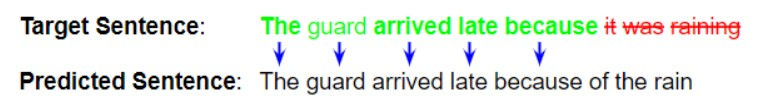
\includegraphics[scale=0.8]{BLEU_1.jpg}
            \caption{Precision 1-grams}

        \end{figure}

        Precision 1-grams = 5/8

        \item Precision 2-grams:
        
        \begin{figure}[h!] \centering

            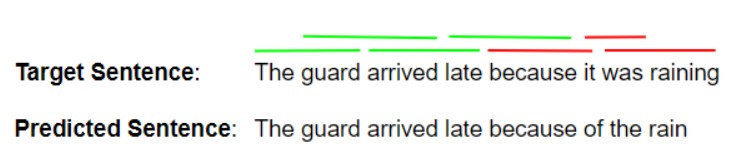
\includegraphics[scale=0.8]{BLEU_2.jpg}
            \caption{Precision 2-grams}

        \end{figure}

        Precision 2-grams = 4/7

        \item Precision 3-grams:
        
        \begin{figure}[h!] \centering

            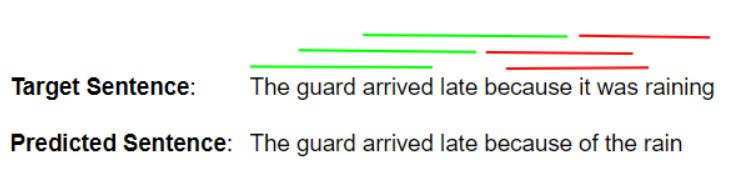
\includegraphics[scale=0.8]{BLEU_3.jpg}
            \caption{Precision 3-grams}

        \end{figure}

        Precision 3-grams = 3/6

        \item Precision 4-grams:
        
        \begin{figure}[h!] \centering

            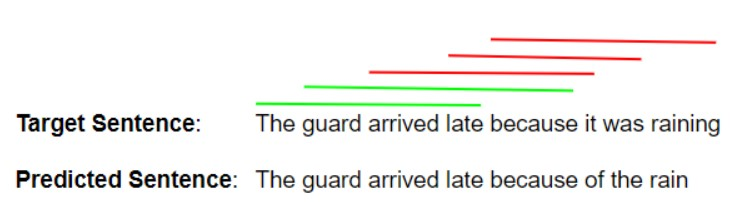
\includegraphics[scale=0.8]{BLEU_4.jpg}
            \caption{Precision 4-grams}

        \end{figure}
        
        Precision 4-grams = 2/5

    \end{itemize}

    Bước 2: Tính Brevity Penalty:

    \begin{equation}
        \mathrm{BP}=\exp\Big(1-\dfrac{r}{c}\Big)=\exp\Big(1-\dfrac{8}{8}\Big)=1
    \end{equation}

    Bước 3: Tính độ chính xác trung bình hình học $\mathrm{GAP}(N)$:

    \begin{equation}
        \mathrm{GAP}(N)=\exp\big( \sum_{n=1}^N w_n \log p_n \big)=\prod_{i=1}^N p_n^{w_n}=\Big(\dfrac{5}{8}\dfrac{4}{7}\dfrac{3}{6}\dfrac{2}{5}\Big)^{\dfrac{1}{4}}\approx 0.516973
    \end{equation}

    Bước 4: Tính BLEU score:

    \begin{equation}
        \mathrm{BLEU}(N)=\mathrm{BP}.\mathrm{GAP}(N)\approx 0.516973
    \end{equation}

    \section{Thực nghiệm và kết quả}

    \subsection{Dữ liệu}

    Tập dữ liệu được sử dụng cho quá trình huấn luyện là Flickr30k.
    Tập dữ liệu này gồm khoảng 31 nghìn ảnh được thu thập từ mạng xã hội Flickr, mỗi ảnh đi kèm với 5 câu miêu tả mẫu được con người gán nhãn.
    Flickr30k có một tập dữ liệu thu nhỏ là Flickr8k với chỉ 8 nghìn ảnh.

    Ngoài ra còn có một tập dữ liệu phổ biến và có kích thước lớn hơn nhiều là COCO Captions với khoảng 118 nghìn ảnh.
    Nhưng do hạn chế về cấu hình máy, tập dữ liệu COCO Captions sẽ không được sử dụng.

    \begin{figure}[h!] \centering

        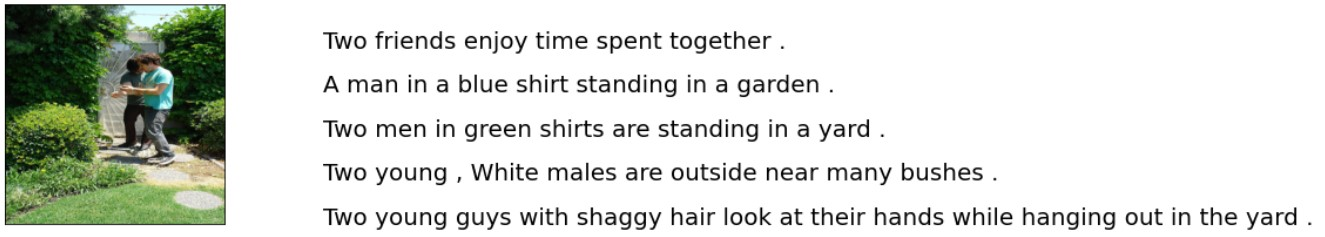
\includegraphics[scale=0.6]{Flickr_Sample_1.jpg}
        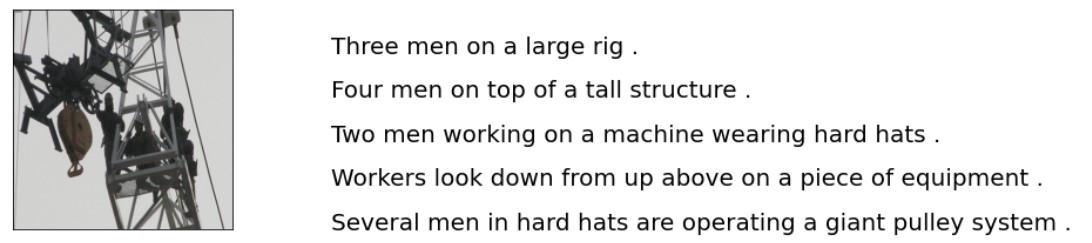
\includegraphics[scale=0.6]{Flickr_Sample_2.jpg}
        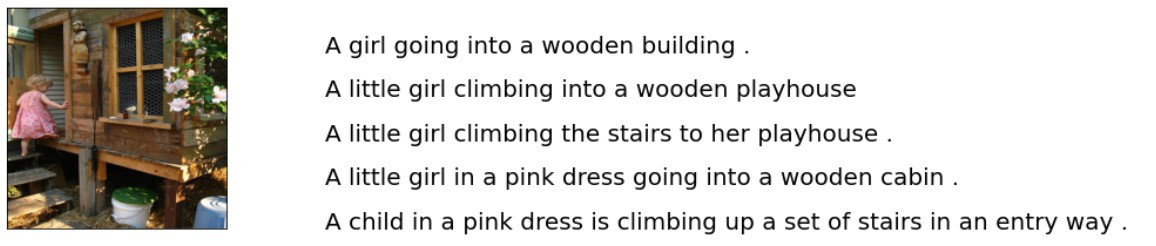
\includegraphics[scale=0.6]{Flickr_Sample_3.jpg}
        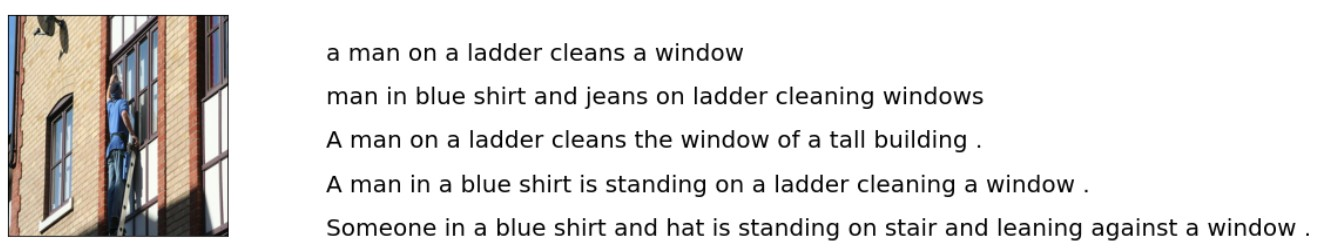
\includegraphics[scale=0.6]{Flickr_Sample_4.jpg}
        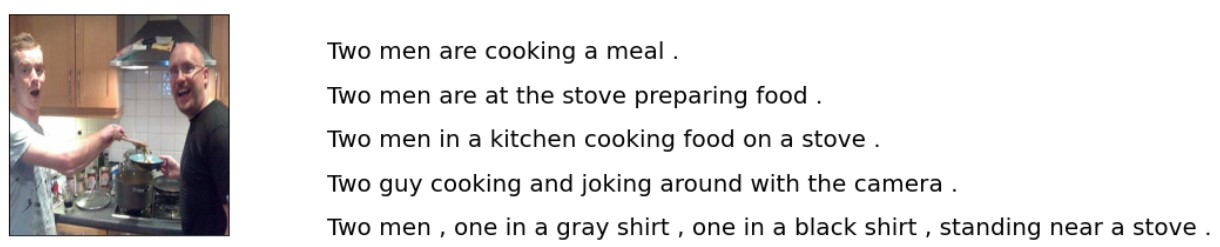
\includegraphics[scale=0.6]{Flickr_Sample_5.jpg}
        \caption{Một số hình ảnh mẫu và câu miêu tả tương ứng}
        \label{fig:Flickr30k-Sample-Image}

    \end{figure}

    
    \begin{figure}[h!] \centering

        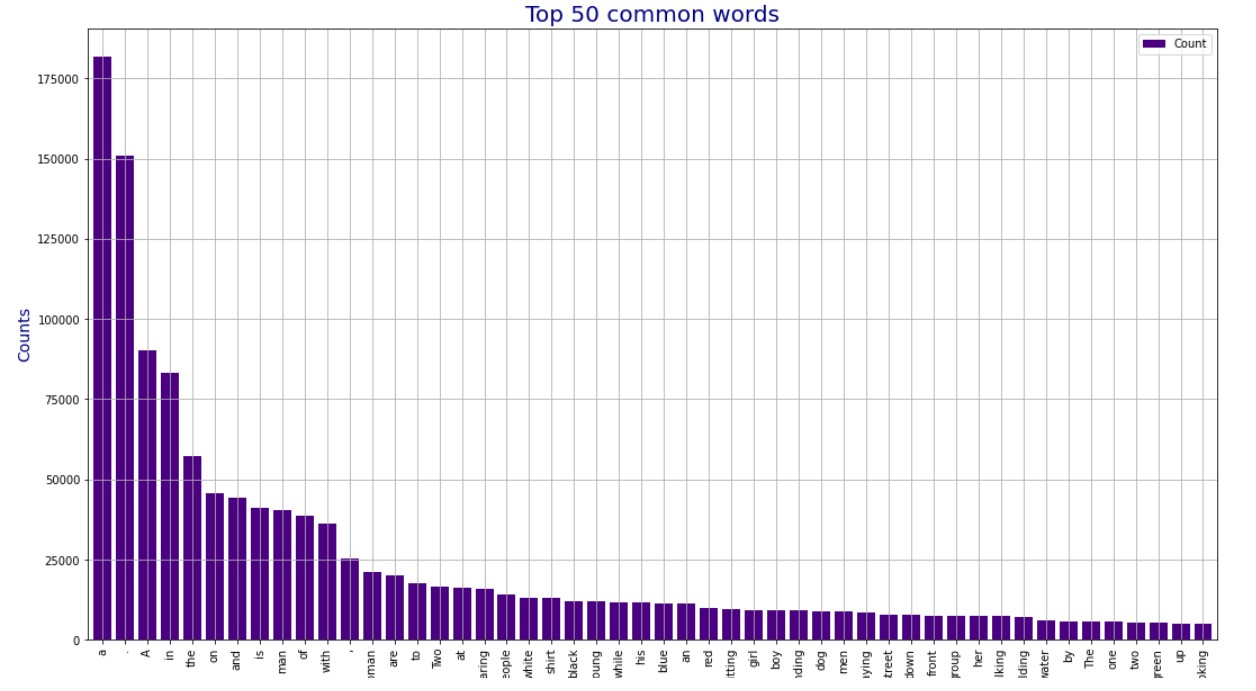
\includegraphics[scale=0.5]{Flickr_frequency_raw_word.jpg}
        \caption{Một số hình ảnh mẫu và câu miêu tả tương ứng}
        \label{fig:Flickr_frequency_raw_word}

    \end{figure}

    Hình \ref{fig:Flickr_frequency_raw_word} hiển thị tần số xuất hiện của các từ trong tập dữ liệu. Ta nhận thấy từ "a", "A" và dấu chấm là 3 từ được xuất hiện nhiều nhất.
    Ta nhận thấy có vấn đề nếu không tiền xử lý dữ liệu, nhiều từ bản chất có cùng nghĩa nhưng lại được xem là hai từ khác nhau. Ta cần biến đổi chúng về cùng một từ gốc (ví dụ "a" và "A" thành "a").

    \begin{figure}[h!] \centering

        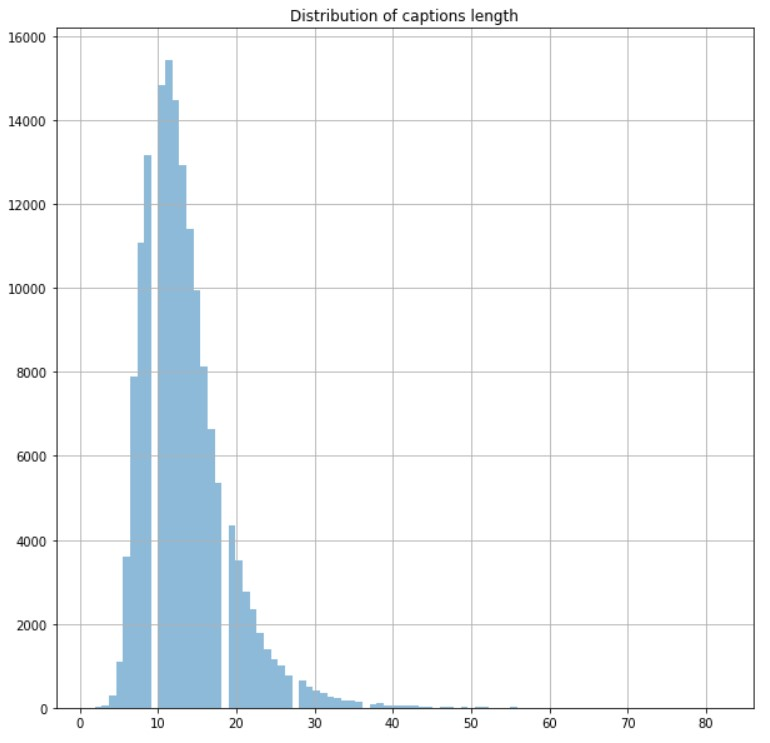
\includegraphics[scale=0.5]{Flickr_Length_Distribution.jpg}
        \caption{Histogram độ dài của các câu miêu tả mẫu}
        \label{fig:Flickr_Length_Distribution}

    \end{figure}

    Hình \ref{fig:Flickr_Length_Distribution} hiển thị histogram độ dài của các câu miêu tả mẫu.
    Ta nhận thấy độ của của các câu miêu tả anh có phân phối lệch phải. Đa số các câu có độ dài từ 5 đến 20 từ.
    Câu có độ dài lớn nhất khoảng 80 từ.

    Ta xử lý dữ liệu văn bản bằng ba bước:

    \begin{itemize}
        \item Chuyển chữ viết hoa thành viết thường.
        \item Xóa cả các dấu tách câu.
        \item Bỏ đi các từ có chứa chữ số.
    \end{itemize}

    Sau tiền xử lý, tần số các từ được hiển thị trong hình \ref{fig:Flickr_frequency_processed_word}. Một số từ xuất hiện rất nhiều như "a", "in", "the", "on", "and", "man",...

    \begin{figure}[h!] \centering

        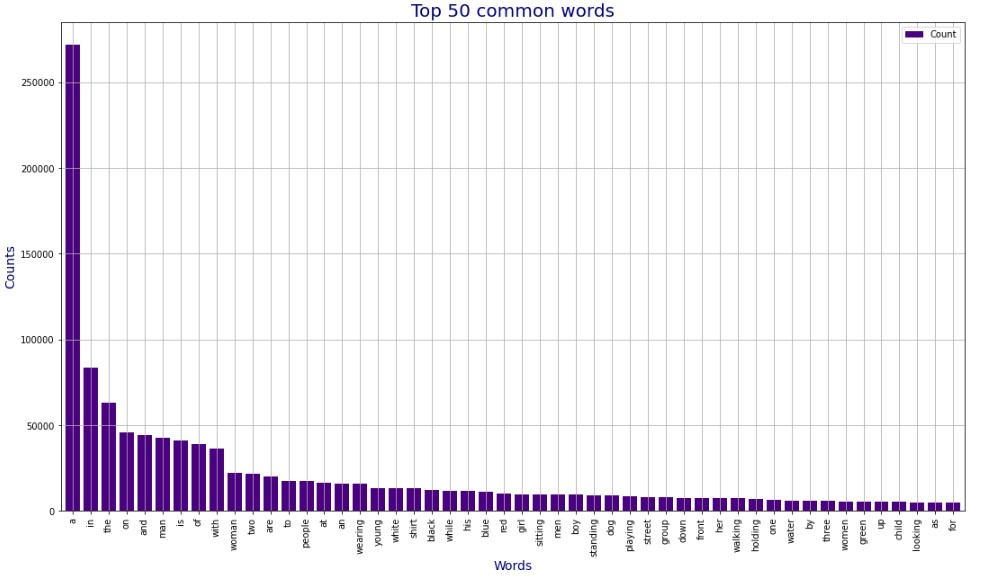
\includegraphics[scale=0.5]{Flickr_frequency_processed_word.jpg}
        \caption{Histogram độ dài của các câu miêu tả mẫu}
        \label{fig:Flickr_frequency_processed_word}

    \end{figure}

    \subsection{Thực thi}

    Mô hình được thực thi sử dụng framework PyTorch. 
    PyTorch là một machine learning framework mã nguồn mở dựa trên thư viện Torch được ra mắt vào tháng 9 năm 2016, được sử dụng cho các ứng dụng thị giác máy tính và xử lý ngôn ngữ tự nhiên.

    PyTorch có một hệ sinh thái rất lớn các công cụ và thư viện đi kèm:
    \begin{itemize}
        \item Flair
        \item ParlAI
        \item OpenMMLab
        \item FastAI
        \item Vissl
        \item AllenNLP
    \end{itemize}

    \subsubsection{Encoder}

    Encoder sử dụng pretrained ResNet-101 \cite{he2016deep} bỏ hai lớp cuối (lớp pooling và lớp phân loại).
    Thêm một lớp AdaptiveAvgPool2d để cố định kích thước của feature map đầu ra là [14, 14, 2048]

    \begin{figure}[h!] \centering

        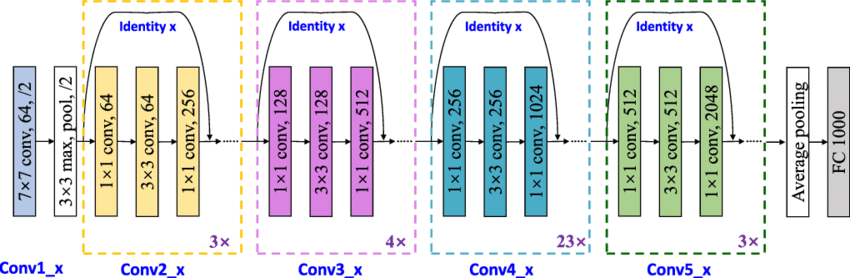
\includegraphics[scale=0.5]{ResNet-101-based-deep-feature-extractor.png}
        \caption{Cấu trúc ResNet-101}
        \label{fig:ResNet-101-based-deep-feature-extractor}

    \end{figure}

    ResNet là kiến trúc được sử dụng phổ biến nhất ở thời điểm hiện tại. 
    ResNet cũng là kiến trúc sớm nhất áp dụng batch normalization. 
    Mặc dù là một mạng rất sâu khi có số lượng layer lên tới 152 nhưng nhờ áp dụng những kỹ thuật đặc biệt mà ta sẽ tìm hiểu bên dưới nên kích thước của ResNet50 chỉ khoảng 26 triệu tham số. 
    Kiến trúc với ít tham số nhưng hiệu quả của ResNet đã mang lại chiến thắng trong cuộc thi ImageNet năm 2015.

    Những kiến trúc trước đây thường cải tiến độ chính xác nhờ gia tăng chiều sâu của mạng CNN. 
    Nhưng thực nghiệm cho thấy đến một ngưỡng độ sâu nào đó thì độ chính xác của mô hình sẽ bão hòa và thậm chí phản tác dụng và làm cho mô hình kém chính xác hơn. 
    Khi đi qua quá nhiều tầng độ sâu có thể làm thông tin gốc bị mất đi thì các nhà nghiên cứu của Microsoft đã giải quyết vấn đề này trên ResNet bằng cách sử dụng kết nối tắt.

    Các kết nối tắt (\textit{skip connection}) giúp giữ thông tin không bị mất bằng cách kết nối từ layer sớm trước đó tới layer phía sau và bỏ qua một vài layers trung gian.
    ResNet có khối tích chập (Convolutional Bock, chính là Conv block trong hình) sử dụng bộ lọc kích thước $3 \times 3$. 
    Khối tích chập bao gồm 2 nhánh tích chập trong đó một nhánh áp dụng tích chập $1 \times 1$ trước khi cộng trực tiếp vào nhánh còn lại.

    \begin{figure}[h!] \centering

        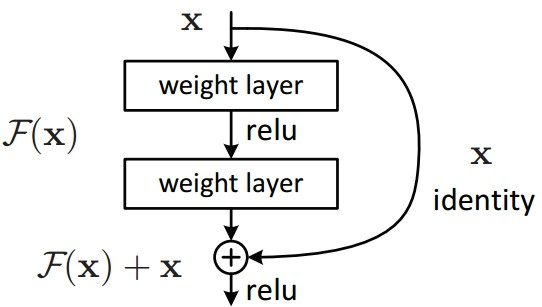
\includegraphics[scale=0.6]{Residual_Block.jpg}
        \caption{Residual Block}
        \label{fig:Residual_Block}

    \end{figure}

    Giả sử ta có $\bold{x}$ là đầu vào của khối xác định (\textit{Indentity Block}). Ta cần ánh xạ đầu vào $\bold{x}$ thành hàm $f(\bold{x})$. 
    Để tìm ra ánh xạ chuẩn xác tương đương với hàm $f(\bold{x})$ là một việc khá khó. 
    Nhưng nếu cộng thêm ở đầu ra thành $\bold{x} + f(\bold{x})$ thì ta sẽ quy về tham số hóa độ lệch, tức cần tham số hóa phần dư $f(\bold{x})$.
    Tìm ánh xạ theo phần dư sẽ dễ hơn nhiều vì chỉ cần tìm giá trị $f(\bold{x})$ sao cho nó gần bằng 0 là có thể thu được một ánh xạ chuẩn tắc.
    Tại một khối xác định, chúng ta sẽ áp dụng một hàm kích hoạt ReLU sau mỗi xen kẽ giữa những tầng trọng số. 
    Mặc dù có kiến trúc khối kế thừa lại từ GoogleNet nhưng ResNet lại dễ tóm tắt và triển khai hơn rất nhiều vì kiến trúc cơ sở của nó chỉ gồm các khối tích chập và khối xác định.
    
    \subsubsection{Mô hình Attention}

    Mô hình Attention là một mạng MLP đơn giản. 
    Đầu tiên các vector gán nhãn $\bold{a}_i$ được biến đổi về số chiều attention là 512.
    Trạng thái $\bold{h}_{t-1}$ cũng được biến đổi về số chiều attention là 512. Cộng các vector trên (cần có broadcasting).
    Sau đó biến đổi kết quả này về số chiều bằng 1. Áp dụng hàm softmax để tạo ra attention map $\alpha_{ti}$.

    \subsubsection{Decoder}

    Các câu mẫu và ảnh tương ứng sẽ được sắp xếp theo thứ tự giảm dần độ dài câu mẫu như hình \ref{fig:Padded_Pack_Sequence}.
    Hệ quả là mỗi timestep sẽ có một batchsize riêng và khi timestep tăng batchsize không tăng so với timestep trước.
    Đây là một kỹ thuật giúp xử lý các timestep dễ dàng hơn và tận dụng tốt hơn hiệu năng của phần cứng.

    \begin{figure}[h!] \centering

        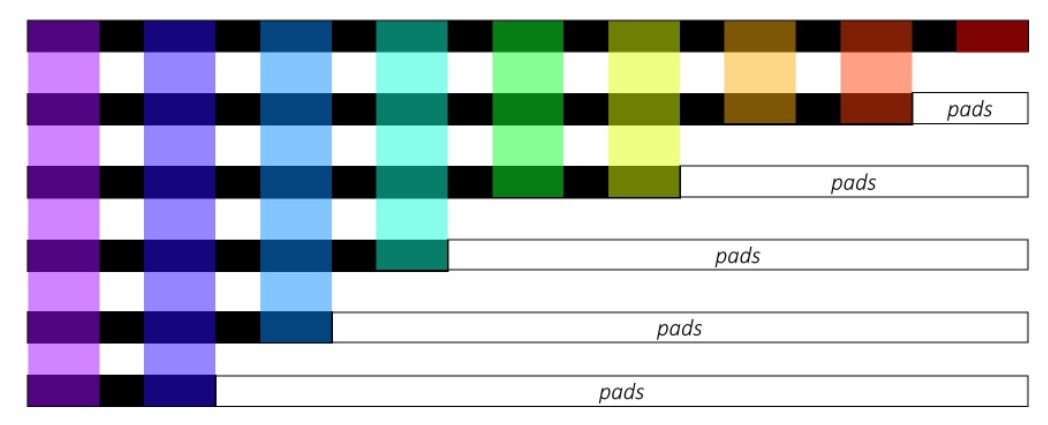
\includegraphics[scale=0.6]{Padded_Pack_Sequence.jpg}
        \caption{Các câu mẫu được sắp xếp theo thứ tự không tăng về độ dài}
        \label{fig:Padded_Pack_Sequence}

    \end{figure}

    Mỗi timestep sẽ tính lại Attention map $\lbrace \alpha_{ti} \rbrace$ và vector bối cảnh $\hat{\bold{z}}_t$. 
    Tại mỗi timestep, đầu vào của LSTM là ghép của vector bối cảnh $\hat{\bold{z}}_t$ và vector embedding của từ kết quả ngay timestep liền kề trước $\bold{Ey}_{t-1}$.

    \subsubsection{Tiền xử lý ảnh}

    Bước tiền xử lý ảnh được thực hiện như trong quá trình train pretrained ResNet-101:
    \begin{itemize}
        \item Ảnh được resize về kích thước $256 \times 256$
        \item Được xử lý qua công thức:
        \begin{equation}
            \dfrac{\mathrm{image}/255-[0.485, 0.456, 0.406]}{[0.229, 0.224, 0.225]}
        \end{equation}
    \end{itemize}

    \subsubsection{Các siêu tham số quá trình huấn luyện}

    Các siêu tham số được sử dụng cho quá trình huấn luyện:

    \begin{itemize}
        \item Optimizer: Adam Optimizer
        \item Batch size: 32
        \item Encoder learning rate: 2e-5
        \item Decoder learning rate: 4e-4
        \item Attention dimension: 512
        \item Decoder dimension: 512
        \item Số từ trong từ điển: 10000
        \item Metrics: BLEU-4
        \item Reduce learning rate on plateau: giảm 0.8 sau 8 epoch không có sự cải thiện BLEU-4
        \item Môi trường huấn luyện: Kaggle Kernel
        \item Loss: Cross Entropy và Attention Regularization
    \end{itemize}

    \subsubsection{Kỹ thuật chọn từ}

    \begin{enumerate} [label=(\alph*)]
        \item Greedy Search

        Kỹ thuật Greedy Search là tại mỗi timestep, từ được dự đoán chính là từ có xác xuất đầu ra lớn nhất.
        Đây là một kỹ thuật rất đơn giản, nhanh hay được sử dụng. 
        Nhưng có một nhược điểm là không phải lúc nào tại mỗi bước chọn từ có xác suất đầu ra lớn nhất thì cả câu dự đoán là một câu hợp lý nhất.

        \item Beam Search
        
        Beamseach là một kỹ thuật phổ biến trong các kiến trúc seq2seq hiện đại. 
        Trong các bài toán xử lý ngôn ngữ như dịch máy, sinh mô tả ảnh, tóm tắt văn bản, tổng hợp tiếng nói,... yêu cầu đầu ra của mô hình là chuỗi các từ có trong từ điển.

        Mỗi từ trong chuỗi từ mà mô hình dự đoán sẽ đi kèm theo một phân phối xác suất tương ứng.
        Khi đó, Decoder sẽ dựa trên phân phối xác suất đó để tìm ra câu phù hợp nhất.

        Tìm kiếm câu phù hợp nhất yêu cầu ta duyệt qua tất cả các câu có thể có từ dự đoán của mô hình.
        Thường thì tử điển có kích thước khá lớn khoảng từ 10000 đến 30000 từ. Vì vậy không gian tìm kiếm sẽ rất lớn là kích thước từ điển lũy thừa với độ dài của câu dự đoán.

        Do không gian tìm kiếm là quá lớn. Thực tế ta thường dùng một thuật toán tìm kiếm heuristic để có được một kết quả tìm kiếm đủ tốt cho mỗi dự đoán thay vì phải tìm kiếm toàn cục.

        Mỗi câu sẽ được gán một số điểm dựa trên xác suất phân phối của chúng, thuật toán tìm kiếm sẽ dựa trên số điểm này để đánh giá các chuỗi từ này.

        Beam search có một siêu tham số là $k$ là số từ khiến tổ hợp từ có tổng xác suất tích lũy lớn nhất trong quá trình dịch.

        Ta xét ví dụ, ta cần dịch câu \textit{"Tôi sẽ về thăm ba mẹ ở Việt Nam"}, giả sử ta đặt $k=3$ và tập từ vựng tiếng Anh chứa 10000 từ.

        \textbf{Bước 1:} Tìm ra 3 từ có xác suất lớn nhất ứng với đầu vào

        \begin{itemize}
            \item Khi đưa đầu vào mã hóa vào Decoder, mô hình sẽ dùng hàm softmax lên toàn bộ 10000 từ.
            \item Trong 10000 khả năng, mô hình lựa chọn 3 từ có xác suất lớn nhất.
            \item Lưu 3 từ có xác suất lớn nhất vào bộ nhớ. Ví dụ 3 từ đó là \textit{I, My, We}
        \end{itemize}

        \begin{figure}[h!] \centering

            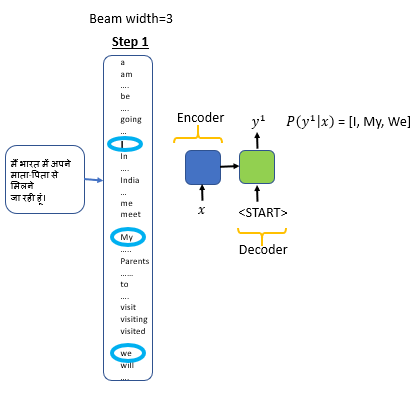
\includegraphics[scale=0.5]{Beam_search_2.png}
            \caption{Beam search bước 1}
            \label{fig:Beam_search_2}
    
        \end{figure}
        

        \textbf{Bước 2:} Tìm ra 3 cặp gồm từ đầu tiên và từ thứ hai có xác suất có điều kiện lớn nhất

        \begin{itemize}
            \item Lấy 3 từ \textit{I, My, We} từ bước 1 bổ sung đầu vào cho bước 2.
            \item Dùng hàm softmax lên 10000 từ để tìm ra 3 từ tốt nhất cho bước 2. Việc lựa chọn này có xét đến xác suất có điều kiện giữa từ đầu tiên và từ thứ 2.
            \item Giả sử 3 cặp có xác suất cao nhất là \textit{I am, My parents, I will}. Chúng ta loại bỏ từ \textit{We} vì nó không còn xuất hiện trong bước này.
            \item Tại mỗi bước, ta khởi tạo 3 bản sao của mạng để đánh giá đầu ra. Số lượng bản số bằng với tham số $k$.
        \end{itemize}

        \begin{figure}[h!] \centering

            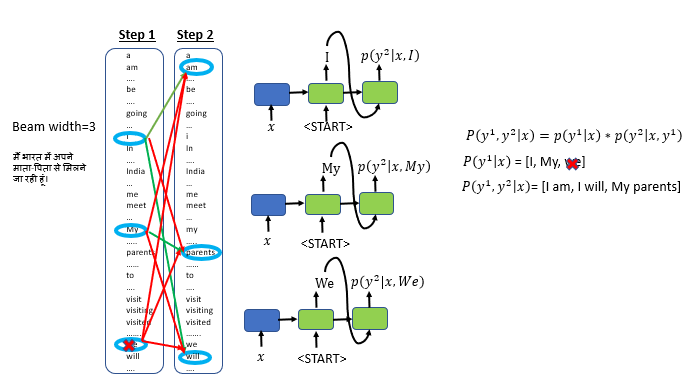
\includegraphics[scale=0.5]{Beam_search_3.png}
            \caption{Beam search bước 2}
            \label{fig:Beam_search_3}
    
        \end{figure}

        \textbf{Bước 3:} Xác định từ thứ 3 tương tự như bước 2

        \begin{itemize}
            \item Từ cặp từ đầu tiên \textit{I am, My parents, I will}, tìm ra từ thứ 3 với xác suất cao nhất.
            \item Giả sử ta có 3 ứng viên tốt nhất là \textit{I am visiting, I will visit, I am going}, ta loại bỏ \textit{My parents} khỏi tập ứng viên.
        \end{itemize}

        \begin{figure}[h!] \centering

            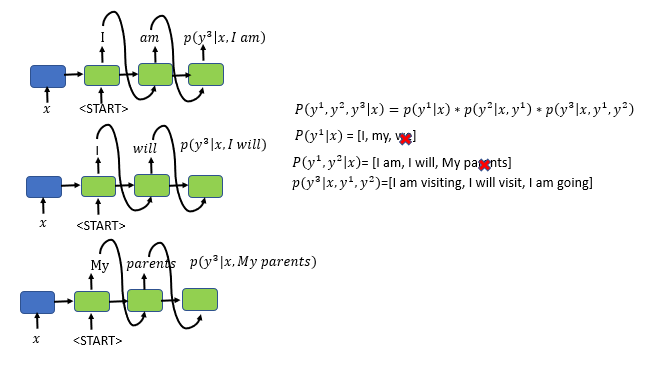
\includegraphics[scale=0.5]{Beam_search_4.png}
            \caption{Beam search bước 3}
            \label{fig:Beam_search_4}
    
        \end{figure}

        Ta tiếp tục quá trình cho đến khi có được 3 ứng viên hoàn chỉnh với các xác suất có điều kiện tương ứng.
        Ta sẽ chọn ra ứng viên có xác suất cao nhất làm đầu ra cuối cùng

        \begin{table}[h!]
            \centering\begin{tabular}{|l|l|}
            \hline
            Câu & Xác suất \\ \hline
            I am going to meet my parents in Vietnam & \textbf{0.72} \\ \hline
            I am visiting my parents in Vietnam & 0.67 \\ \hline
            I will visit Vietnam to meet my parents & 0.62 \\ \hline
            \end{tabular}
            \caption{Các câu ứng viên và xác suất tương ứng}
        \end{table}

        Giá trị $k$ càng lớn, khả năng ta có một câu đầu ra tốt là cao hơn nhưng cũng tốn nhiều bộ nhớ và năng lực tính toán hơn.

    \end{enumerate}

    \subsection{Kết quả}

    Hình \ref{fig:Loss} biểu diễn giá trị Loss function theo epoch.
    Tại khoảng epoch thứ 5 loss function đạt giá trị nhỏ nhất sau đó tăng dần.
    Đây là dấu hiệu cho thấy hiện tượng overfitting đã xuất hiện.
    Nguyên nhân của việc này là số epoch giảm learning rate khi BLEU Score không cải thiện quả lớn.
    Khiến cho Loss function tăng dần lên. Đến epoch 12, quá trình train dừng do Kaggle Kernel giới hạn thời gian chạy một phiên (\textit{Session}).

    \begin{figure}[h!] \centering

        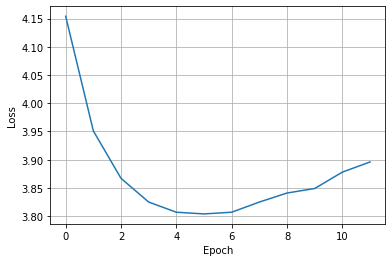
\includegraphics[scale=0.6]{Loss.png}
        \caption{Loss function theo epoch}
        \label{fig:Loss}

    \end{figure}

    Hiện tượng tương tự cũng xảy ra với BLEU Score.

    \begin{figure}[h!] \centering

        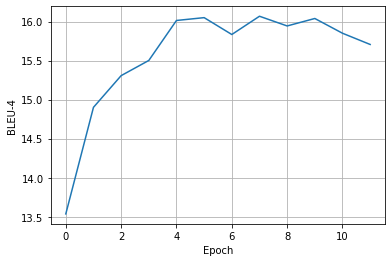
\includegraphics[scale=0.6]{BLEU-4.png}
        \caption{BLEU Score theo peoch}
        \label{fig:BLEU-4}

    \end{figure}

    Khó khăn trong quá trình huấn luyện: Thiết bị hạn chế (30 tiếng một tuần) khiến cho khó có đủ thời gian để lựa chọn các bộ tham số tối ưu, 
    cũng như thời gian huấn luyện cho phép đủ dài để có thể quan sát quá trình huấn luyện một cách toàn diện nhất.

    Một số hiển thị về Attention map $\lbrace \alpha_{ti} \rbrace$ được hiển thị trong các hình 

    \begin{figure}[h!] \centering

        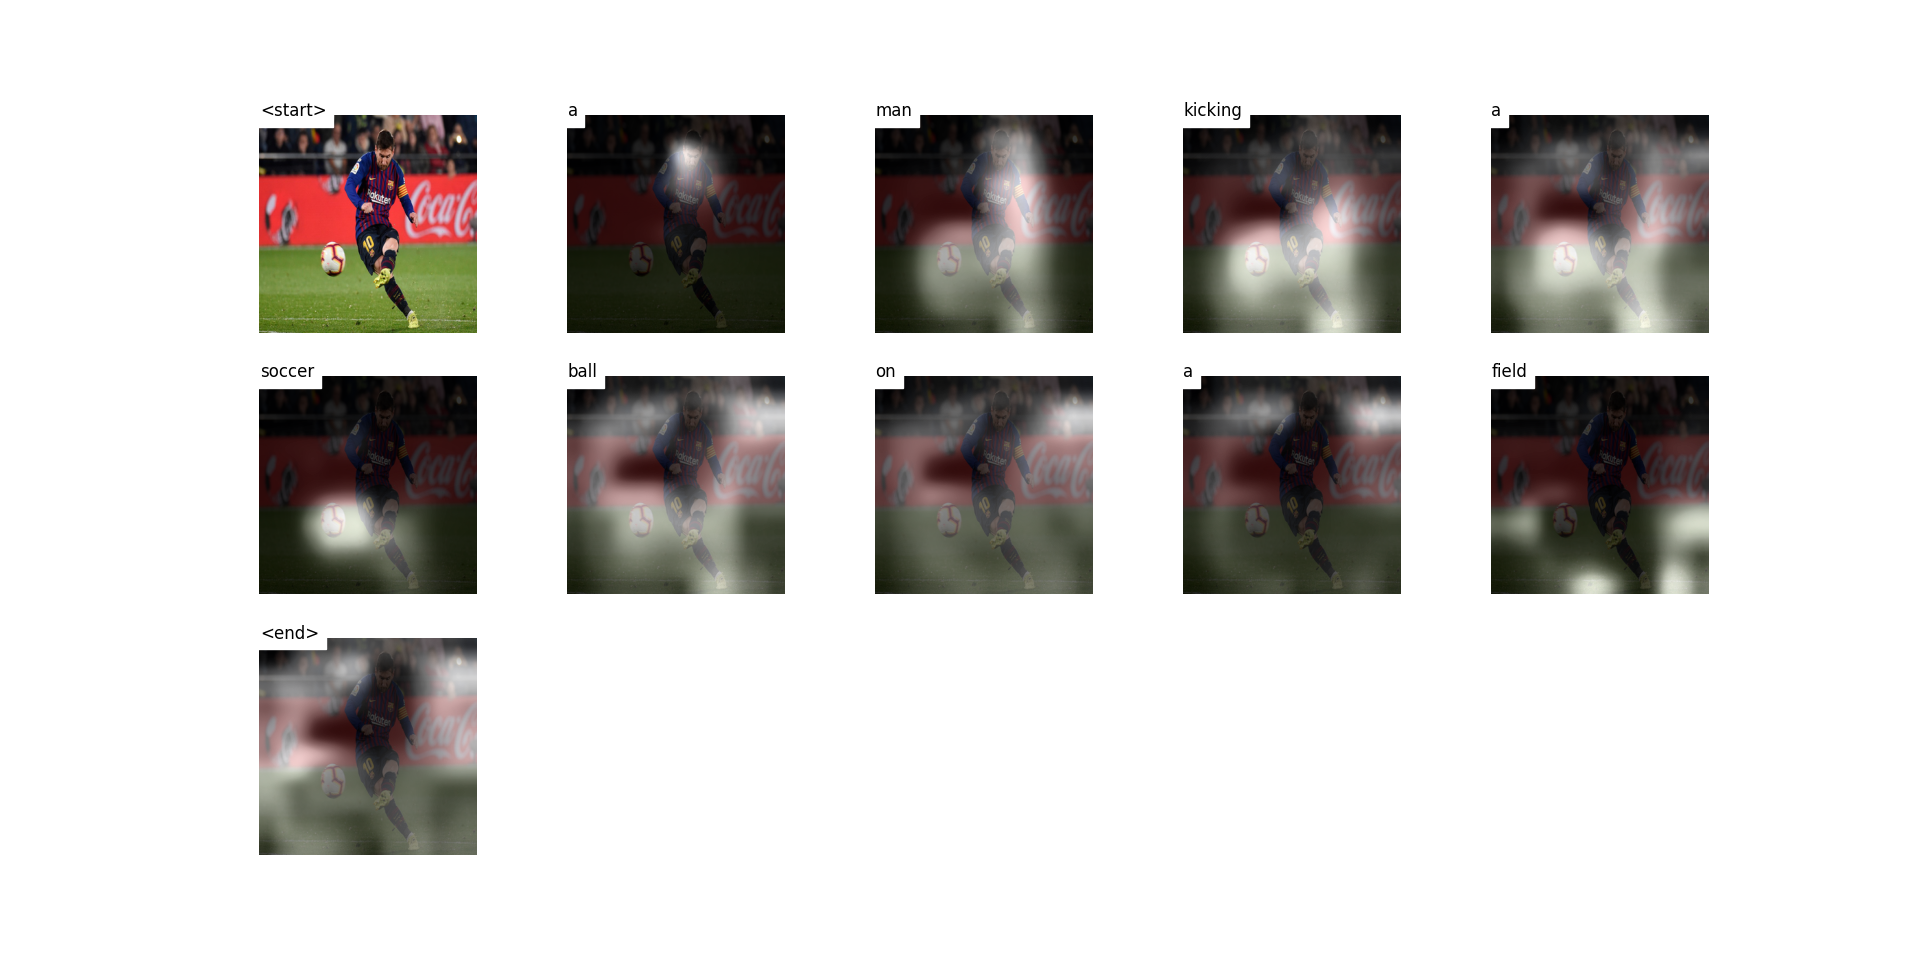
\includegraphics[scale=0.3]{Attention_Sample_1.png}
        \caption{Biểu diễn Attention Map theo từng timestep}
        \label{fig:Attention_Sample_1}

    \end{figure}

    \begin{figure}[h!] \centering

        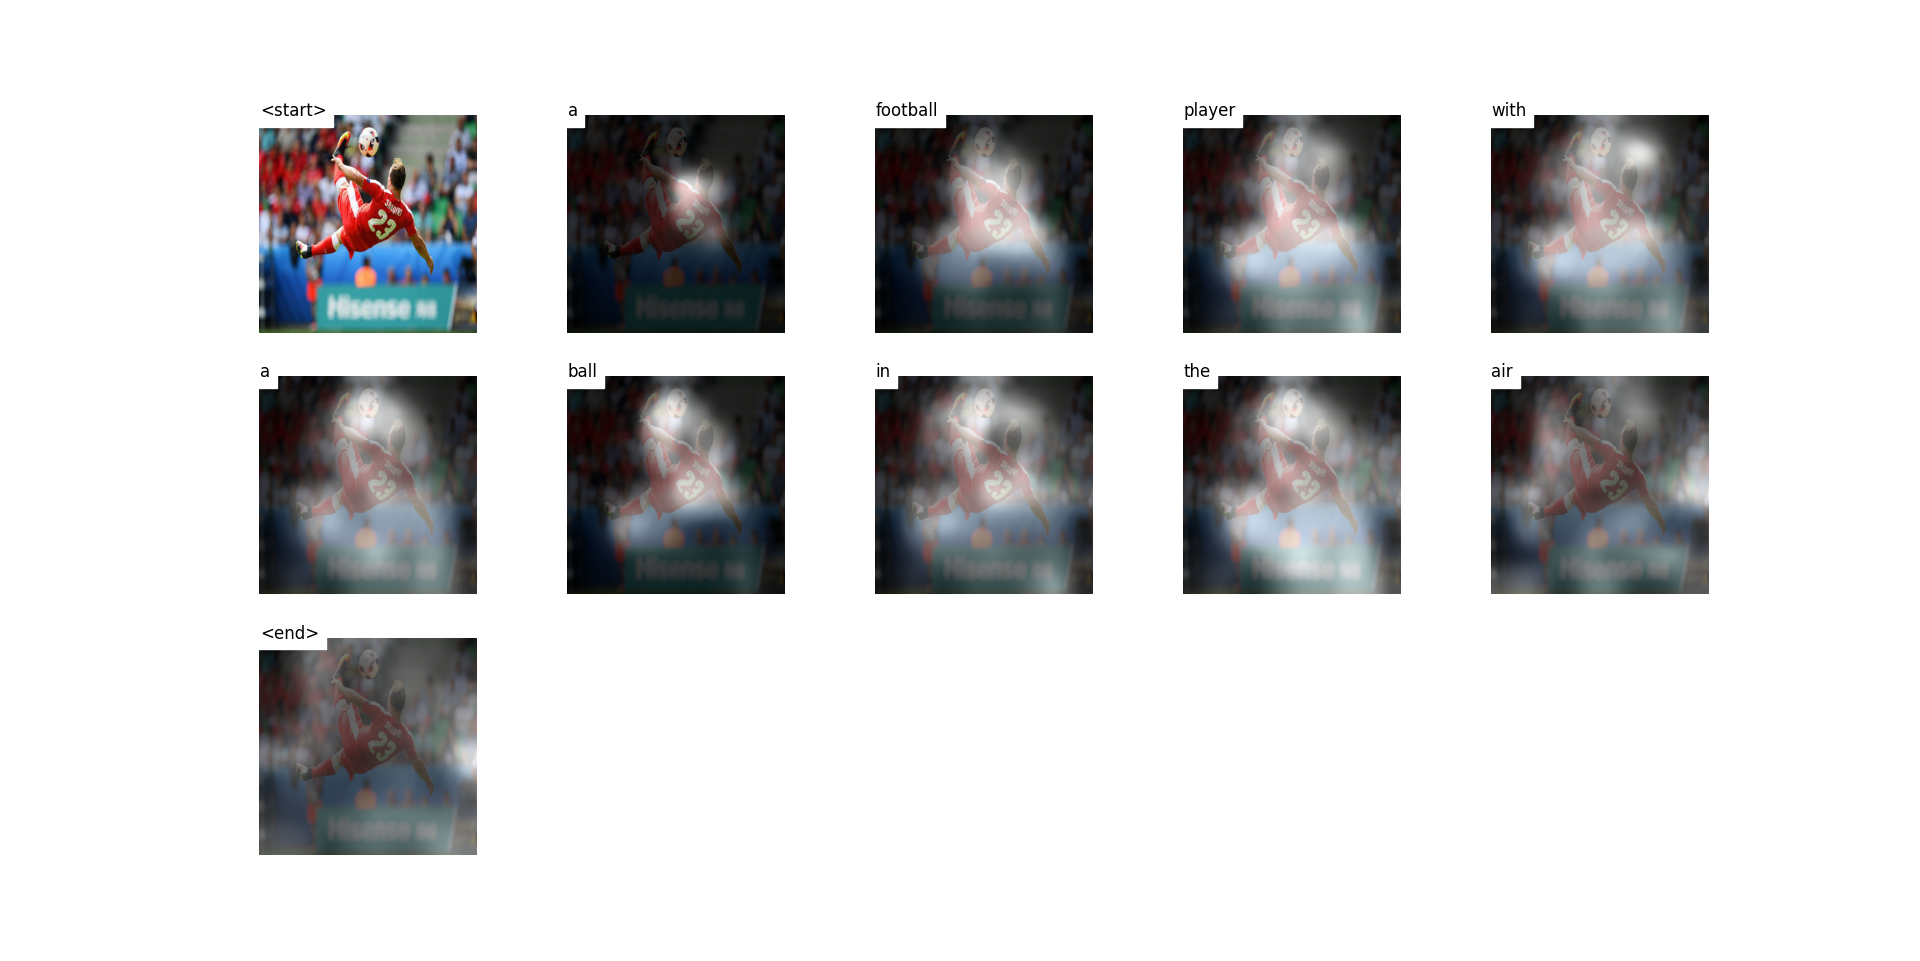
\includegraphics[scale=0.3]{Attention_Sample_2.png}
        \caption{Biểu diễn Attention Map theo từng timestep}
        \label{fig:Attention_Sample_2}

    \end{figure}
    
    \section{Demo giao diện}
    
    Để xây dựng giao diện người dùng, thư viện được sử dụng là PyQt5.
    PyQt là một bộ công cụ tiện ích GUI (\textit{Graphical User Interface}). 
    Đây là Python interface cho Qt, một trong những thư viện GUI đa nền tảng mạnh mẽ và phổ biến nhất. 
    PyQt được phát triển bởi RiverBank Computing Ltd.

    PyQt API là một tập hợp các mô-đun chứa một số lượng lớn các lớp và hàm. 
    Module QtCore chứa chức năng không phải GUI để làm việc với tệp và thư mục. 
    Module QtGui chứa tất cả các lớp và hàm về giao diện. Ngoài ra, có các mô-đun để làm việc với XML (QtXml), SVG (QtSvg) và SQL (QtSql),...

    Một số module thường xuyên được sử dụng:

    \begin{itemize}
        \item QtCore: các lớp không phải GUI được sử dụng bởi các module khác.
        \item QtGui: Các thành phần giao diện người dùng.
        \item QtMultimedia: Các lớp lập trình đa phương tiện cấp thấp.
        \item QtNetwork: Các lớp lập trình mạng.
        \item ...
    \end{itemize}

    \begin{figure}[h!] \centering

        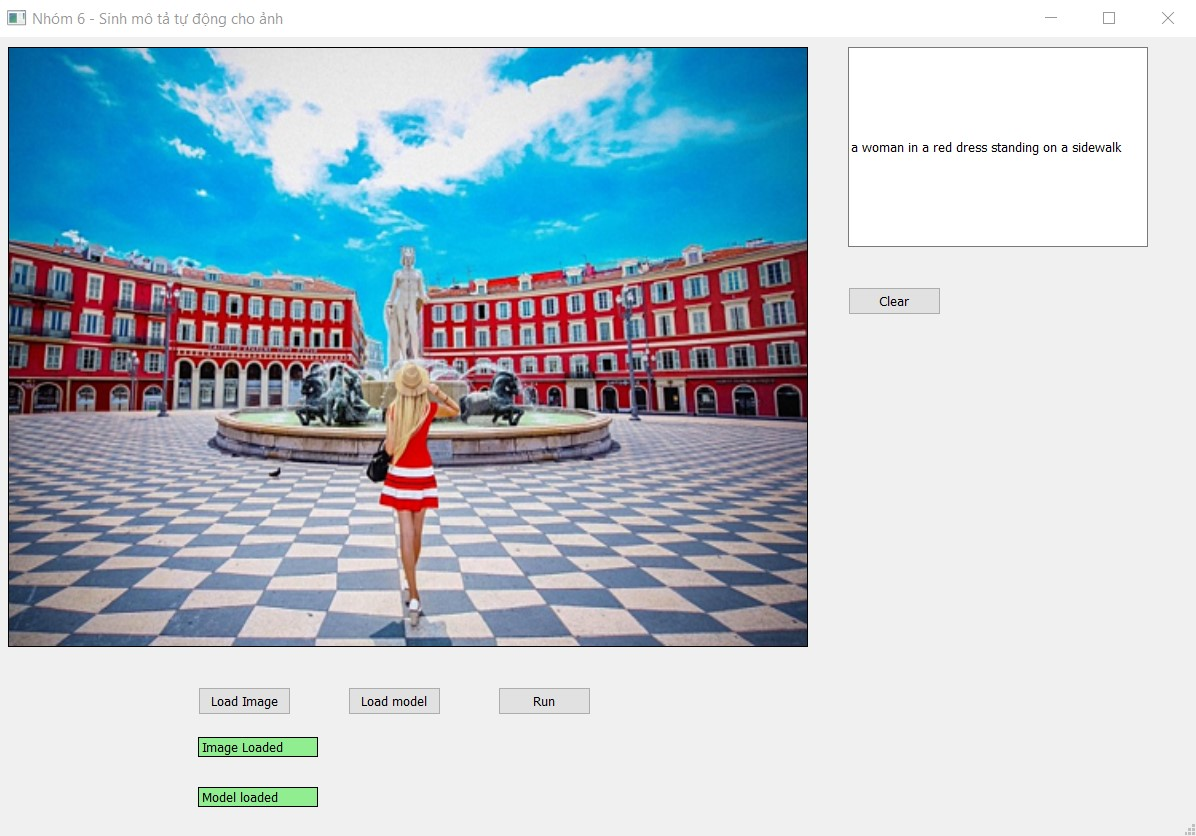
\includegraphics[scale=0.5]{UI.jpg}
        \caption{Giao diện phần mềm}
        \label{fig:UI}

    \end{figure}

    Pipeline của quá trình thực hiện phần mềm:

    \begin{itemize}
        \item Ấn nút "Load model"
        \item Ấn nút "Load Image" và chọn ảnh cần được sinh mô tả
        \item Ấn nút "Run" và kết quả sẽ hiện trên ô textbox góc trên bên phải của giao diện
    \end{itemize}

    Nếu ta muốn xóa tất cả chữ ở trong ô textbox kết quả, ta ấn nút "Clear". 
    Hoặc nếu muốn sinh mô tả cho một ảnh khác chỉ cần ấn "Load Image" và chọn lại ảnh. 
    Nút "Load model" chỉ cần ấn một lần để khởi tạo model.
    \newpage
    \section{Kết luận và hướng phát triển đề tài}

    Đề tài đã trình bày lý thuyết cơ bản về dịch máy, mô hình sinh mô tả ảnh và lý thuyết cơ chế Attention.
    Những điểm đã đạt được:

    \begin{itemize}
        \item Hiểu được lý thuyết dịch máy
        \item Hiểu được mô hình sinh mô tả ảnh
        \item Các mô hình cơ chế Attention
        \item Xây dựng được mô hình sinh mô tả Ảnh
        \item Xây dựng được giao diện người dùng
    \end{itemize}

    Tuy nhiên đề tài vẫn còn một số những hạn chế nhất định, do hạn chế về mặt thời gian và thiết bị phần cứng nên đề tài chưa thể huấn luyện mô hình để có kết quả tốt.
    Đề tài chưa đề cập đến các thành tựu các các kiến trúc mô hình sinh mô tả ảnh gần đây. Ở các bước phát triển tiếp theo đề tài sẽ phát triển theo các hướng:

    \begin{itemize}
        \item Sử dụng các pretrained word embedding như: GLOVE, CRAWL, GoogleNews, NumberBatch, Paragram-300, ... 
        \item Sử dụng các cấu trúc sinh mô tả ảnh hiện đại sử dụng Transformer \cite{vaswani2017attention}. 
        Xu hướng các mô hình mô tả ảnh hiện đại không còn sử dụng Encoder mã hóa toàn bộ thông tin từ ảnh mà sẽ chỉ trích xuất các đặc trưng ở các vùng nhất định, mỗi vùng này sẽ được xem như là một từ ở phần đầu vào của Encoder trong bài toán dịch máy.
        Một số phương pháp điển hình của phương pháp này là: VL-T5 \cite{cho2021unifying}, Oscar \cite{li2020oscar}, VinVL \cite{zhang2021vinvl}, LXMERT \cite{tan2019lxmert}, M2-Transformer \cite{cornia2020meshed}.
    \end{itemize}

    \newpage
    \addcontentsline{toc}{section}{TÀI LIỆU THAM KHẢO}
    %\bibliographystyle{IEEEtraN}
    %\bibliography{ref}
    %\pagestyle{plain}
    \printbibliography[title={TÀI LIỆU THAM KHẢO}]

    %\newpage
    %\printbibliography
\end{document}
